\documentclass [PhD] {uclathes}

\usepackage{amsthm}
\usepackage{amsmath}
\usepackage{amssymb}
\usepackage{bbm}
\usepackage{mathtools}
\usepackage{subfigure}
\usepackage{placeins}
\usepackage{import}
\usepackage{graphicx}
\usepackage{todonotes}
\usepackage{color}
\usepackage{array}
\usepackage{natbib}
\usepackage[toc,page]{appendix}
\usepackage{floatrow}
\usepackage{color, colortbl}
\usepackage{placeins} % for FloatBarrier
\usepackage{algorithm}
\usepackage{algorithmic}
\usepackage{chapterbib}
\definecolor{Gray}{gray}{0.9}
\DeclareMathAlphabet{\mbf}{OT1}{ptm}{b}{n}

\theoremstyle{definition}
\newtheorem{example}{Example}[section]
\newtheorem{definition}{Definition}[section]
\newtheorem{conj}{Conjecture}[section]
\newtheorem{lemma}{Lemma}[section]
\newtheorem{prop}{Proposition}[section]
\newtheorem{notation}{Notation}
\def\newblock{\hskip .11em plus .33em minus .07em}

\graphicspath{{}}
\makeatletter
\newcommand\appendtographicspath[1]{%
  \g@addto@macro\Ginput@path{#1}%
}
\makeatother

\def\p{\ensuremath{\mathbf{p}}}
\def\v{\ensuremath{\mathbf{v}}}
\def\x{\ensuremath{\mathbf{x}}}
\def\one{\mathbbm{1}}
\def\eps{\varepsilon}

\def\RR{\mathbb{R}}
\def\HH{\mathbb{H}}
\def\PP{\mathbb{P}}
\def\NN{\mathbb{N}}
\def\EE{\mathbb{E}}
\def\II{\mathbb{I}}

\def\A{\mathcal{A}}
\def\Y{\mathcal{Y}}
\def\O{\mathcal{O}}
\def\U{\mathcal{U}}
\def\P{\mathcal{P}}
\def\I{\mathcal{I}}
\def\L{\mathcal{L}}
\def\D{\mathcal{D}}
\def\V{\mathcal{V}}
\def\C{\mathcal{C}}
\def\R{\mathcal{R}}
\def\S{\mathcal{S}}
\def\T{\mathcal{T}}

\def\del{\partial}
\def\1{^{\prime}}
\def\neg{\mathord{\sim}}
\def\qtx#1{\quad\text{#1}\quad}
\def\subs{\subseteq}
\def\andn{\smallsetminus}

\def\IPV{\I_{\operatorname{Poisson}}}


%opening
\def\sscale{0.7}
%\def\tT{\widetilde\T}
\def\tT{\T\1}

\def\nop{\text{nop}}
\def\ang#1{\left\langle#1\right\rangle}
\def\inv{^{-1}}

\def\seq{\operatorname{Sequences}}
\def\Rep{\operatorname{Rep}}
\def\Comp{\operatorname{Comp}}
\def\Adj{\operatorname{Adj}}

\renewcommand{\algorithmicrequire}{\textbf{Input:}}
\renewcommand{\algorithmicensure}{\textbf{Output:}}                         % personal LaTeX macros

%%%%%%%%%%%%%%%%%%%%%%%%%%%%%%%%%%%%%%%%%%%%%%%%%%%%%%%%%%%%%%%%%%%%%%
%
% Usually things live in separate flies.
%
% \input {prelim}                           % preliminary page info

%%%%%%%%%%%%%%%%%%%%%%%%%%%%%%%%%%%%%%%%%%%%%%%%%%%%%%%%%%%%%%%%%%%%%%%%
%                                                                      %
%                          PRELIMINARY PAGES                           %
%                                                                      %
%%%%%%%%%%%%%%%%%%%%%%%%%%%%%%%%%%%%%%%%%%%%%%%%%%%%%%%%%%%%%%%%%%%%%%%%

\title          {Models and Methods for Sensor-Based Environment Exploration
% Modeling and Optimization for Environment Exploration from Sensory Data
% Algorithms for Scene Exploration and Representation
% Optimization Schemes for Scene Exploration in Robotics and Vision
% ...
}
\author         {Joshua Anthony Hernandez}
\department     {Mathematics}
\degreeyear     {2015}

%%%%%%%%%%%%%%%%%%%%%%%%%%%%%%%%%%%%%%%%%%%%%%%%%%%%%%%%%%%%%%%%%%%%%%%%

\chair          {Stefano Soatto}
\member         {Joseph Teran}
\member         {Rafail Ostrovsky}
\member         {Luminita Vese}


%%%%%%%%%%%%%%%%%%%%%%%%%%%%%%%%%%%%%%%%%%%%%%%%%%%%%%%%%%%%%%%%%%%%%%%%

%\dedication     {\textsl{To my mother \ldots \\}}

%%%%%%%%%%%%%%%%%%%%%%%%%%%%%%%%%%%%%%%%%%%%%%%%%%%%%%%%%%%%%%%%%%%%%%%%

%\acknowledgments {(Acknowledgments omitted for brevity.)}

%%%%%%%%%%%%%%%%%%%%%%%%%%%%%%%%%%%%%%%%%%%%%%%%%%%%%%%%%%%%%%%%%%%%%%%%

% UCLA Policy on Vita
% For security reasons, UCLA policy specifies that your birth year and birth place should not be included in your vita.
%               
\vitaitem{2012--2015}{Graduate Student Researcher, {\textsl UCLA Vision Lab}.
 \begin{itemize}
  \item {\textsl Information-Driven Exploration of Ising-Modeled Terrain } \\
  Developed a method for efficiently exploring and mapping highly-occluded environments,
  choosing informative viewpoints using a  prior on terrain shape and an efficiently-computed approximation of joint measurement entropy. 
  \item {\textsl Visual-Inertial Navigation} \\ 
  Implemented efficient numerical methods for the Corvis visual-inertial navigation system.
  Analyzed the ambiguity inherent in visual-inertial sensor fusion systems, and characterised the set
  of indistinguishable trajectories.
  \item {\textsl Representation Reduction for Autonomous Agents} \\
  Developed and analyzed algorithms for the lossless compresssion of an autonomous agent's belief state, 
  modulo a given task, with the aim of reducing memory and computational requirements.
 \end{itemize}
}
 
\vitaitem{Summer 2011}{Summer Intern, {\textsl Instruments Division, Jet Propulsion Lab}.  Contributed to the onboard image processing system of MSPI (Multiangle SpectroPolarimetric Imager) Satellite.
Identified and eliminated an unusual striping artifact characteristic of that system.
Advisor: Veljko Jovanovich.}
\vitaitem{2005--2011}
{Teaching Assistant, {\textsl UCLA Mathematics}.
Held twice-weekly discussions for several lower-and upper-division classes, to wit: Precalculus, Calculus 1 \& 2, Differential Equations, Complex Analysis, 
Introductory C++, Algorithms and Data Structures, Advanced A \& DS.}

%%%%%%%%%%%%%%%%%%%%%%%%%%%%%%%%%%%%%%%%%%%%%%%%%%%%%%%%%%%%%%%%%%%%%%%%

\publication{J. Dong, N. Karianakis, D. Davis, {\textsl J. Hernandez}, J. Balzer and S. Soatto. Multi-view Feature Engineering and Learning. {\textsl Proc.\ IEEE Conference on Computer Vision and Pattern Recognition (CVPR)}, June 2015.}
\publication{{\textsl J. Hernandez}, K. Tsotsos and S. Soatto. Observability, Identifiability and Sensitivity of Vision-Aided Inertial Navigation. {\textsl Proc.\ International Conference on Robotics and Automation (ICRA)}, May 2015.  {\textsl Best Paper, ICRA 2015}}
\publication{J. Helton, D. McAllaster, {\textsl J. Hernandez}. Non-Commutative Harmonic and Subharmonic Polynomials. {\textsl Integral Equations and Operator Theory}, May 2008, Vol.\ 61, Iss.\ 1, pp 77-102.}

%%%%%%%%%%%%%%%%%%%%%%%%%%%%%%%%%%%%%%%%%%%%%%%%%%%%%%%%%%%%%%%%%%%%%%%%

% 
%%%%%%%%%%%%%%%%%%%%%%%%%%%%%%%%%%%%%%%%%%%%%%%%%%%%%%%%%%%%%%%%%%%%%%%%

\begin {document}
\makeintropages

%%%%%%%%%%%%%%%%%%%%%%%%%%%%%%%%%%%%%%%%%%%%%%%%%%%%%%%%%%%%%%%%%%%%%%
%
% Ordinarily each chapter (at least) is in a separate file.
%
\graphicspath{{Exploration/IDE/}{Exploration/Model/}{Exploration/Implementation/}{Exploration/Horizon/}{Exploration/Suff_Explor/}{Exploration/Eval/}{Exploration/Speedup/}{Exploration/Statistics/}{MinRep/}{SolidObjects/cvpr2014_solobj/}}
\chapter{Representations of the Environment for Robotics Applications}
The work in the following chapters addresses different aspects of the problem of autonomous interaction of a robot with physical environment.
The need for such autonomous capabilities is evident - autonomous vehicles, drones,  and robots, ar safer than  humans to drive, can replace humans where tasks are dangerous, boring, etc.
There are great difficulties in this work, however. We know how to build robots, sensors, control etc., 
but we do not know how to endow a robot with a ``sense'' of the surrounding environment. 
%This is called a representation. It is what is needed to interact with physical space.
%We define a representation as a function of data that supports tasks.
\iffalse
\begin{enumerate}
\item what data? Vision (bearing) and/or range (radar, lidar etc.)
\item what tasks? Simplest ``go to point A'' more complex one could be ``find object X''
\item what is needed for the task: 
\fi
This sense could be a sense of geometry (where is point A? relative to which reference frame? what is a path to A, are there ``obstacles''? what are ``obstacles''),
localization (where are you in relation to obstacles?), topology (what paths are traversable?), photometry (what is an ``object''? How do I find it? 
%This relates to the burgeoning literature on visual search and computer vision
).
Instead of tackling the problem of autonomous interaction head-on, we have focused on a few subproblems.

\section{Summary of core results}
\begin{enumerate}
\item \label{bullet: slam} First: localization. To interact with the environment, first you need to know where you are relative to it. Fundamental problem studied for many years; Observability of the undelying dynamical model is a necessary condition for ANY algorithm to work, in the sense of yielding a unique point estimate. Our contribution is to show that all existing analysis of observability was flawed, and propose new analysis that shows that, contrary to popular belief, pose is not observable from visual and inertial sensors. However, we show that the ambiguous set is bounded, and compute it analytically.
\item \label{bullet: SO} Second: Once I know where I am, I need to know what is around me. This is a problem called ``mapping''. Building geometric maps (point clouds) well explored problem. However, to interact intelligently need more than point cloud, need topology. How is the world around us divided into ``objects''? Chapter 4 talks about a way of organizing points into surfaces and then connected components of surfaces, that can be considered ``objects'' for the purpose of interaction, from video.
\item \label{bullet: exploration} Once I know where I am and have a model of the (Visible) environment, with respect to which I know the location of an object of interest (point A), I need to know how to get to point A, which may not be visible. This requires exploration. Chapter 1 deals with this problem. The contribution is an efficient algorithm with provable bounds on the exploration time and amenable to be extended to non-compact domains (relevant in vision because one can see to infinity).
\item \label{bullet: rep-redux} To explore the boundaries of this problem set, we also ask whether a representation is needed at all, at least for simple problems like going to point A. To this end, we explore the possibility of directly encoding/representing/optimizing the map from sensory data to control action, designed so as to achieve the goal (of getting to point A).
\end{enumerate}

\iffalse TODO: finish this
\section{State of the art}

Vast literature. For \ref{bullet: slam} there are books, dedicated conferences, problem known as SLAM in robotics, SFM in computer vision, activities since the early 1900 (see intro to textbook MASKS). State-of-the-art (see observability paper), was upended by our results (best paper at ICRA)

For \ref{bullet: SO} considerable amount of work on obtaining sparse maps (subject of textbooks, e.g. MASKS); also consierable effort in fitting surfaces from point clouds (see Virginia's papers references). Relatively less effort in organizing such surfaces into ``layers'' or objects. See Chan-Adelson ``layers'', then detachable object detection, most recently deep learning,  but we are interested in partitioning the scene, rather than the image.

For \ref{bullet: exploration} lots of work on planning, also textbook (see LaValle), relatively few work on planning under uncertainty (but still massive literature). in our case most of the uncertainty is due to visibility (or lack thereof), relatively fewer works, but see work of Landa, Osher, Tsai, etc. Take that as starting point, see references therein

%for \ref{bullet: rep-redux} this relates to work in computer science theory, although in a simplified setting where the target cannot move (lest it is considerably more complex, turns into a game), related literature on pursuit-evasion games etc.
\fi

\section{Overview of the thesis}
This work is organized as follows: Chapter 2 analyzes the problem of localization using monocular video and inertial sensors.
Chapter 3 deals with the problem of segmenting 3D pointclouds into task-relevant ``objects''.
Chapter 4 explores the problem of efficient autonomous mapping using range sensors.
Chapter 5 looks into schemes for reducing the computational overhead required to maintain an agent's
awareness relative to a task.

\chapter{Observability of Visual-Inertial Navigation}
\newcommand{\be}{\begin{equation}}
\newcommand{\ee}{\end{equation}}
\newcommand{\ba}{\left[ \begin{array}}
\newcommand{\ea}{\end{array} \right]}
\newcommand{\bea}{\begin{eqnarray}}
\newcommand{\eea}{\end{eqnarray}}
\newcommand{\bc}{\begin{cases}}
\newcommand{\ec}{\end{cases}}
\newcommand{\psfigure}[3]
        {
        \begin{tabular}{c}
        { \psfig{figure=#1,height=#2in,width=#3in}}
        \end{tabular}   }

\def\real{\mathbb{R}}
\def\X{{\mathbf{X}}}
\def\x{{\mathbf{x}}}
\def\w{\omega}
\def\hw{{\widehat\w}}
\def\ww{\tilde\w}
\def\hww{\widehat\ww}

\newtheorem{defn}{Definition}
\newtheorem{rem}{Remark}
\newtheorem{theorem}{Theorem}
\newtheorem{claim}{Claim}
\newtheorem{corollary}{Corollary}

\def\gw{\tilde{g}}
\def\Xw{\tilde{X}}
\def\Rw{\tilde{R}}
\def\Tw{\tilde{T}}
\def\1{^{\prime}}

\def\g{g}
\def\inv{^{-1}}
\def\RR{\mathbb{R}}
\def\s{\sigma}
\def\sit{\s_{i}}
%\def\dot#1{\tfrac{d#1}{dt}}
\def\dX{\delta X}
\def\subs{\subset}
\def\andn{\smallsetminus}
\def\Mm{\mathcal{M}}
\def\SO{\operatorname{SO}}
\def\SE{\operatorname{SE}}
\def\so{\mathfrak{so}}
\def\se{\mathfrak{se}}
\def\Aa{\mathcal{A}}
\def\ignore#1{}
\def\imu{_\mathrm{imu}}
\def\m{{m}}
\def\M{{M}}
\def\I{\mathcal{I}}

%\def\cut#1{{ #1}}
\def\cut#1{{}}

%\begin{abstract}
%\end{abstract}

\section{Introduction}
Visually-aided navigation (bearing), and range-aided navigation (radar) can be framed as a filtering problem. The model is non-linear, has unknown parameters, and unknown inputs ({\em e.g.,} accelerometer and gyrometer bias derivative), typically treated as driving noise in a random walk model.
Observability is a necessary condition for {\em any} filter/observer to operate, hence a literature on observability analysis of visually-aided navigation \cite{kellyS09,mourikisR07,jonesS07}. Relatively little on range-aided. 
Unknown parameters are typically included in the state, thus transforming an identification problem into a filtering one, and their identifiability analysis lumped in the observability analysis of the resulting (augmented) model.
Noise does not affect the observability of a model, so for the purpose of observability analysis, they are set to zero. This is because, by assumption, noise is ``uninformative:'' It is typically modeled as a realization of a white zero-mean, homoscedastic process, independent of the state of the model.
However, the driving input to the random walk model of accelerometer and gyro bias is typically small but {\em not} independent of the state. In fact, far from being uninformative, it is strongly correlated with it, as it is its temporal derivative. Thus, it should be treated as an {\em unknown input}, rather than a ``noise.'' As such, it should be included in the observability/identifiability analysis. 
Our first contribution is to show that while (a prototypical model of) assisted navigation and auto-calibration is {\em observable} in the absence of unknown input, it is {\em not} observable when unknown inputs are taken into account. This exposes a methodological flaw with the observability analysis of assisted navigation in the existing literature.
Our second contribution is to reframe observability as a {\em sensitivity} analysis, and to show that while the set of indistinguishable trajectories is {\em not} a singleton (as it would be if the model was observable), but it is nevertheless bounded to a set. We explicitly characterize this set and show that, interestingly, it may not contain the ``true'' state trajectory. Finally, we provide bounds on the volume of this subset as a function of the characteristics of the unknown inputs.
We do so for bearing-only augmentation, range-only augmentation, and combined augmentation.
Rather than study observability of linearized system, or algebraically checking the rank conditions, that offers no insight on the structure of the indistinguishable states, we characterize observability directly in terms of indistinguishable sets.
\subsection{Notation}

A reference frame is represented by an orthogonal $3\times 3$ positive-determinant (rotation) matrix $R \in \SO(3) \doteq \{ R \in \real^{3\times 3} \ | \ R^T R = R R^T = I, \ {\operatorname{det}}(R) = +1\}$ and a translation vector $T \in \real^3$. They are collectively indicated by $g = (R, T) \in \SE(3)$. When $g$ represents the change of coordinates from a reference frame ``a'' to another (``b''), it is indicated by $g_{ba}$. Then the columns of $R_{ba}$ are the coordinate axes of $a$ relative to the reference frame $b$, and $T_{ba}$ is the origin of $a$ in the reference frame $b$. If $p_a$ is a point relative to the reference frame $a$, then its representation relative to $b$ is $p_b = g_{ba} p_a$. In coordinates, if $X_a$ are the coordinates of $p_a$, then $X_b = R_{ba}X_a + T_{ba}$ are the coordinates of $p_b$. 

A time-varying pose is indicated with $g(t) = (R(t), T(t))$ or $g_t = (R_t, T_t)$, and the entire trajectory from an initial time $t_i$ and a final time $t_f$ $\{g(t) \}_{t = t_i}^{t_f}$ is indicated in short-hand notation with $g_{t_i}^{t_f}$; when the initial time is $t_0 = 0$, we omit the subscript and call $g^{t}$ the trajectory ``up to time $t$''. The time-index is sometimes omitted for simplicity of notation when it is clear from the context.

We indicate with $\widehat V = (\widehat \w, v) \in \se(3)$ the (generalized) velocity or ``twist'', where $\widehat \w$ is a skew-symmetric matrix $\widehat \w \in \so(3) \doteq \{S \in \real^{3\times 3} \ | \ S^T = -S\}$ corresponding to the cross product with the vector $\w \in \real^3$, so that $\widehat \w v = \w \times v$ for any vector $v\in \real^3$. We indicate the generalized velocity with $V = (\w, v)$. We indicate the group composition $g_1 \circ g_2$ simply as $g_1 g_2$. 
In homogeneous coordinates, $\bar X_b = G_{ba} \bar X_a$ where $\bar X^T = [X^T \ 1]$ and 
\begin{equation}
G \doteq \ba{cc} R & T \\ 0 & 1 \ea \in \real^{4\times 4}
~~~~
\hat V \doteq \ba{cc} \widehat \w & v \\ 0 & 0 \ea.
\end{equation}
Composition of rigid motions is then represented by matrix product.


\subsection{Mechanization Equations}

The motion of a sensor platform is represented as the time-varying pose $g_{sb}$ of the body relative to the spatial frame. To relate this to measurements of an inertial measurement unit (IMU) we compute the temporal derivatives of $g_{sb}$, which yield the (generalized) body velocity $V_{sb}^b$, defined by $\dot g_{sb}(t) = g_{sb}(t) {\widehat V}^b_{sb}(t)$, which can be broken down into the rotational and translational components $\dot R_{sb}(t) = R_{sb}(t) \widehat{\w}_{sb}^b(t)$ and $\dot T_{sb}(t) = R_{sb}(t) v_{sb}^b(t)$. An ideal gyrometer (gyro) would measure $\w\imu  = \w_{sb}^b$. The translational component of body velocity, $v_{sb}^b$, can be obtained from the last column of the matrix $\frac{d}{dt} {\widehat V}^b_{sb}(t)$. That is, $ \dot{v}_{sb}^b = \dot{R_{sb}^T}\dot T_{sb} + R_{sb}^T \ddot T_{sb} = - \widehat{\w}_{sb}^b v_{sb}^b + R_{sb}^T \ddot T_{sb} \doteq - \widehat{\w}_{sb}^b v_{sb}^b + \alpha_{sb}^b $, which serves to define $\alpha_{sb}^b \doteq R_{sb}^T \ddot T_{sb}
$. These equations can be simplified by defining a new linear velocity, $v_{sb}$, which is neither the body velocity $v_{sb}^b$ nor the spatial velocity $v_{sb}^s$, but instead $v_{sb} \doteq R_{sb}v_{sb}^b$. Consequently, we have that $ \dot T_{sb}(t) = v_{sb}(t) $ and $ \dot v_{sb}(t) = \dot R_{sb} v_{sb}^b + R_{sb} \dot{v}_{sb}^b = \ddot T_{sb} \doteq \alpha_{sb}(t) $ where the last equation serves to define the new linear acceleration $\alpha_{sb}$; as one can easily verify we have that $ \alpha_{sb} = R_{sb} \alpha_{sb}^b.$ An ideal accelerometer (accel) would then measure  $ \alpha\imu  = R_{sb}^T(t) (\alpha_{sb}(t) - \gamma)$.

There are several reference frames to be considered in an aided navigation scenario. The {\em spatial frame} $s$, typically attached to Earth and oriented so that gravity $\gamma$ takes the form $\gamma^T = [0 \ 0 \ 1]^T \| \gamma \|$ where $\| \gamma \|$ can be read from tabulates based on location and is typically around $9.8m/s^2$. The {\em body frame} $b$ is attached to the IMU.\footnote{In practice, the IMU has several different frames due to the fact that the gyro and accel are not co-located and aligned, and even each sensor (gyro or accel) is composed of multiple sensors, each of which can have its own reference frame. Here we will assume that the IMU has ben pre-calibrated so that accel and gyro yield measurements relative to a common reference frame, the {\em body frame}. In reality, it may be necessary to calibrate the alignment between the multiple-axes sensors (non-orthogonality), as well as the gains (scale factors) of each axis.} The {\em camera frame} $c$, relative to 
which image 
measurements are captured, is also unknown, although we will assume that {\em intrinsic calibration} has ben performed, so that measurements on the image plane are provided in metric units. Finally, the {\em radar frame}, or range frame $r$, is that of the antenna relative to which range measurements are provided.

The equations of motion (known as mechanization equations) are usually described in terms of the body frame at time $t$ relative to the spatial frame $g_{sb}(t)$. Since the spatial frame is arbitrary (other than for being aligned to gravity), it is often chosen to be co-located with the body frame at time $t = 0$. To simplify the notation, we indicate this time-varying frame $g_{sb}(t)$ simply as $g$, and so for $R_{sb}, T_{sb}, \w_{sb}, v_{sb}$, thus effectively omitting the subscript $sb$ everywhere it appears. This yields
\begin{equation}
\begin{cases}
\begin{tabular}{rl}
$\dot T$ &$= V$ \\%~~~~ ~~ T(0) = 0 \\
$\dot R$ &$= R \widehat \w$ \\%~~~~~ R(0) = R_0\\
$\dot V$ &$= \alpha$  \\% ~~~~ ~~~ V(0) = V_0 \\
$\dot \w$ &$= w$ \\
$\dot \alpha$ &$= \xi$
\end{tabular}
\end{cases}
\end{equation}
where $w \in \real^3$ is the rotational acceleration, and $\xi \in \real^3$ the translational jerk (derivative of acceleration). Although $\alpha$ corresponds to neither body nor spatial acceleration, it can be easily related to accel measurements: 
\begin{equation}
\boxed{\alpha\imu (t) = R^T(t) (\alpha(t)- \gamma) + \underbrace{\alpha_b(t) + n_{\alpha}(t)}}
\label{eq-accel}
\end{equation}
where the measurement error in bracket includes a slowly-varying mean (``bias'') $\alpha_b(t)$ and a residual term $n_\alpha$ that is commonly modeled as a zero-mean (its mean is captured by the bias), white, homoscedastic and Gaussian noise process. In other words, it is assumed that $n_\alpha$ is independent of $\alpha$, hence uninformative. Here $\gamma$ is the gravity vector expressed in the spatial frame.\footnote{The orientation of the body frame relative to gravity, $R_0$, is unknown, but can be approximated by keeping the IMU still (so $R^T(t) = R_0$) and averaging the accel measurements, so that $\frac{1}{T}\sum_{t=0}^T \alpha\imu (t)  \simeq  - R_0^T \gamma + \alpha_b$. Assuming the bias to be small (zero), this equation defines $R_0$ up to a rotation around gravity, which is arbitrary. Note that if $\alpha_b \neq 0$, the initial bias will affect the initial orientation estimate.} Measurements from a gyro can be similarly modeled as 
\begin{equation}
\boxed{\w\imu (t) = \w(t) + \underbrace{\w_b(t) + n_{\w}(t)}}
\label{eq-gyro}
\end{equation}
where the measurement error in bracket includes a slowly-varying bias $\w_b(t)$ and a residual ``noise'' $n_\w$ also assumed zero-mean, white, homoscedastic and Gaussian, independent of $\w$.

Other than the fact that the biases $\alpha_b, \w_b$ change {\em slowly}, they can change arbitrarily. One can therefore consider them an {\em unknown input} to the model, or a {\em state} in the model, in which case one has to hypothesize a dynamical model for them. For instance instance
\begin{equation}
\dot \w_b(t) = v_b(t), ~~~ \dot \alpha_b(t) = v_\alpha(t)
\end{equation}
for some unknown input $v_b, v_\alpha$. While it is safe to assume that $v_b, v_\alpha$ are {\em small}, they certainly are not (white, zero-mean and, most importantly) uninformative. Nevertheless, it is common to consider $v_b, v_\alpha$, to be realizations of a Brownian motion that is  {\em independent} of $\w_b, \alpha_b$. This is done for convenience as one can then consider all unknown inputs as ``noise.'' Unfortunately, however, this has repercussion on the analysis of the observability and identifiability of the resulting model (Sect. \ref{sect-bearing-analysis}).

%The resulting model has a {\em state} $x = \{T, R, V\}$ of unknown functions that satisfy a known ordinary differential equation (ODE); unknown but otherwise constant {\em parameters} $p = \{X^i, \gamma\}$, {\em output} measurements $y = \{y^i(t), \alpha(t), \w(t)\}$, {\em noise} terms that are uninformative $n = \{n^i(t), \tilde n_\alpha(t), \tilde n_\w(t)\}$. It then has {\em unknown inputs} $u = \{\alpha_b(t), \w_b(t)\}$. Alternatively, we can consider the biases to be part of the {\em state}, $x = \{T, R, V, \alpha_b, \w_b\}$ and consider the bias derivatives as the unknown inputs $u = \{\dot \alpha_b, \dot \w_b\}$. 

\subsection{Standard and reduced models}

The mechanization equations above define a dynamical model having as output the IMU measurements. Including the initial conditions and biases, we have
\begin{equation}
\begin{cases}
\begin{tabular}{>{$}r<{$} >{$\!\!\!\!\!}l<{$} >{$}r<{$} >{$\!\!\!\!\!}l<{$}}
\dot T &= V & T(0) &= 0 \\
\dot R &= R \widehat \w & R(0) &= R_0\\
\dot V &= \alpha \\ %~~~~~~ V(0) = V_0 \\
\dot \w &= w\\ % ~~~~~~~ \w(0) = \w_0 \\
\dot \alpha &= \xi \\% ~~~~~~ \alpha(0) = \alpha_0 \\
\dot \w_b &= n_{\w_b}  \\
\dot \alpha_b &= n_{\alpha_b}  \\ 
\dot \gamma &= 0 \\
\end{tabular}\\
\begin{tabular}{>{$}r<{$} >{$\!\!\!\!\!}l<{$}}
\w\imu (t) &= \w(t) + \w_b(t) + n_{\w}(t) \\ 
\alpha\imu (t) &= R^T(t) (\alpha(t)- \gamma) + \alpha_b(t) + n_{\alpha}(t) 
\end{tabular}
\end{cases}
\end{equation}
\cut{which is  of  the form\footnote{In fact, if we collect the states into thre groups: Attitude and translational velocity $x_1 \doteq \{T, R, V\} = \{x_{11}, x_{12}, x_{13}\}$; rotational velocity and translational acceleration $x_2 \doteq \{\w, \alpha\} = \{x_{21}, x_{22}\}$ and biases $x_3 \doteq \{\w_b, \alpha_b\} = \{x_{31}, x_{32}\}$, and the IMU measurements $u =\{\w\imu , \alpha\imu \}  = \{u_1, u_2\}$, and gravity as a parameter $p_0 = \gamma$, we have the expression above
%% \begin{equation}
%% \begin{cases}
%% \dot x_1  = f(x_1, x_2)  \\
%% \dot x_2 = n_x \\
%% \dot x_3 = 0 \\
%% y\imu  = h(x_1,x_2, x_3,p_0) + n_y
%% \end{cases}
%% \end{equation}
%% 
where:
\begin{equation}
f(x_1, x_2) = \ba{c} x_{13} \\ x_{12} x_{21} \\ x_{22} \ea ~~
h(x_1, x_2, x_3, p_0) = \ba{c} x_{21} + x_{31} \\ x_{12}^Tx_{22} + x_{32} - x_{12}^T p_0 \ea
\end{equation}
and $n_x = \{w, \xi\}$, $n_y$ are assumed to be realizations of a white, zero-mean, Gaussian random vector. 
Note that the initial conditions are not known, and neither are $w$ and $\xi$. These are conveniently assumed to be white zero-mean Gaussian processes. The biases can be assumed constant in the short term, or an additional noise with small covariance can be added to account for their fluctuation. 
}
\begin{equation}
\begin{cases}
\dot x_1  = f(x_1, x_2)  \\
\dot x_2 = n_x \\
\dot x_3 = n_3 \\
u = h(x_1,x_2, x_3,p_0) + n_y
\end{cases}
\label{eq-standard}
\end{equation}
}
In this standard model, data from the IMU are considered as (output) {\em measurements}. However, it is customary to treat them as (known) {\em input} to the system, by writing $\w$ in terms of $\w\imu $ and $\alpha$ in terms of $\alpha\imu $:
\begin{equation}
\boxed{\w = \w\imu  - \w_b + \underbrace{n_R}_{-n_{\w}}} ~~~~~~ \boxed{\alpha = R(\alpha\imu  - \alpha_b) + \gamma + \underbrace{ n_V}_{- Rn_\alpha}}
\end{equation}
This equality is valid for {\em samples} (realizations) of the stochastic processes involved, but it can be misleading as, if considered as stochastic processes, the noises above are {\em not} independent of the states. Such a dependency, is nevertheless typically neglected. The resulting mechanization model is
\begin{equation}
\boxed{
\begin{cases}
\begin{tabular}{>{$}r<{$} >{$\!\!\!\!\!}l<{$} >{$}r<{$} >{$\!\!\!\!\!}l<{$}}
\dot T &= V &T(0) &= 0 \\
\dot R &= R (\widehat \w\imu  - \widehat \w_b) + n_{R} &R(0) &= R_0\\
\dot V &= R(\alpha\imu  - \alpha_b) + \gamma + n_V \\ %~~~~~~ V(0) = V_0 \\
\dot \w_b &= n_{\w_b} \\
\dot \alpha_b &= n_{\alpha_b}. 
\end{tabular}
\end{cases}
}
\label{eq-mech}
\end{equation}
\cut{
\begin{equation}
{\mathrm %which \ is \ 
of \ the \ form} ~~ 
\begin{cases}
\begin{tabular}{>{$}r<{$} >{$\!\!\!\!\!}l<{$}}
\dot x_1 &= f(x_1, x_3) + g_1(x_1,p_0) \bar u +  g_2(x_1) n_y\\
\dot x_3 &= n_3
\end{tabular}
\end{cases}
\label{eq-reduced}
\end{equation}
where
\begin{equation}
f(x_1,x_3) = \ba{c} x_{13} \\ -x_{12}\widehat x_{31} \\ -x_{12} x_{32} \ea
~~~ g_1(x_1,p_0) \bar u = \ba{ccc} 0 & 0 & 0 \\ x_{12} & 0 & 0\\ 0 & x_{12} & p_0 \ea\ba{c} \widehat u_1 \\ u_2 \\ 1\ea ~~~ g_2(x_1) = \ba{c} 0 \\ x_{12} \\ x_{12} \ea
\end{equation}
This is obtained by solving for $x_2$ as a function of $u$ from the measurement equation of (\ref{eq-standard}) and substituting into the state equation. With an abuse of notation we write this as the ``inverse map'' $x_2 = h^{-1}(u,x_1,x_3,p_0)$. Since $x_{12}^T x_{12} = I$, we can replace $g_2(x_1)$ with $[0 \ I \ I]^T$. %Note that in this case there is no ned to include in the state $\w$ and $\alpha$, since they are measured directly. Also note that there are no outputs (measurements) in this model. If the values of the biases and the noise terms $n_R, n_V$ were known, one could simply integrate the above equations to obtain the trajectory of the state.
%
To simplify the notation, we simply call $u = \{\widehat u_1, u_2, 1\}$ and $n_y = \{0, n_y, n_y\}$, and neglect the dependency on $p_0$, so as to arrive at the expression
\begin{equation}
\begin{cases}
\dot x_1  = f(x_1, x_3) + g_1(x_1)  u +  n_y\\
\dot x_3 = n_3
\end{cases}
\end{equation}
}

\cut{
\subsection{Nominal model}
%
Except for the values of the bias, the above model is just a deterministic integrator with known initial conditions. In the absence of noise and biases, one could simply integrate a {\em nominal model} based on the following equation:
\begin{equation}
{\mathrm NC:}
\begin{cases}
\dot T = V ~~~~ T(0) = 0 \\
\dot R = R \widehat \w\imu   ~~~~~ R(0) = I\\
\dot V = R\alpha\imu + \gamma  ~~~~~~ V(0) = 0
\end{cases}
{\mathrm which \ is \ of \ the \ form} ~~ 
\dot x_1  = f(x_1,0) + g_1(x_1)u 
\label{eq-nominal}
\end{equation}
where $f$ and $g_1$ have the same expression as in (\ref{eq-reduced}). 
We have assumed that $V(0) = 0$, that is, the experiment starts at rest. We call the solution (integration) of the above differential equation the {\em nominal state trajectory} $\hat x = \{ \hat T, \hat R, \hat V\}$.
%
\section{Error-state model (skip)} 
%
If we assume that the nominal state trajectory ${\hat x}^t$ has ben computed we may benefit from writing the actual trajectory $x^t$ as a {\em perturbation} ${\tilde x}^t$ around the nominal trajectory. 
%
If we assume a local coordinate parametrization of $R\in \SO(3)$, for instance the exponential coordinate $\w \in \real^3$ defined by $R = \exp(\widehat \w)$, then $x \doteq \{T(t), \w (t), V(t)\}$ can be written in terms of a {\em nominal state} $\hat x$ obtained by deterministically integrating the nominal model, and the {\em error state} $\tilde x$. Alternatively, the nominal trajectory can be the conditional mean estimated by a filter. In either case, it is possible to write the linearized error state as follows.
%
\subsection{Linearized error-state}
%
If $x = \hat x + \tilde x$, then we have that $f(x,u)$ can be approximated using Taylor Series expansion as:
\begin{equation}
f(x, u)  = f(\hat x, u) + \underbrace{\frac{\partial f}{\partial x}(\hat x)}_{J_f(\hat x,u)}\tilde x + n_f
\end{equation}
with $n_f \in {\mathcal O}(\| \tilde x\|^2)$, where the bracketed matrix is the Jacobian of $f$ computed at the nominal trajectory $\hat x$. It is therefore easy to decouple the evolution $\dot x = f(x, u)$ into the nominal trajectory
\begin{equation}
\dot {\hat x} = f(\hat x, u)
\end{equation}
and the error-state
\begin{equation}
\dot{\tilde x} = J_f(\hat x,u) \tilde x + n_f.
\end{equation}
The advantage of this model is that the latter is a linear time-varying model, for which a standard (linear) Kalman filter can be written. Once the nominal state is integrated and the error state is estimate with a Kalman filter, the actual state trajectory can be approximated by $x = \hat x + \tilde x$.
%
The case of discrete-time is similar: If $x(t+1) = f(x(t), u(t))$ is the evolution of the state, where $u(t)$ is a known input, then it is customary to approximate $x(t+1) \doteq \hat x(t+1) + \tilde x(t+1) = f(\hat x(t), u(t)) + \frac{\partial f}{\partial x}(\hat x,u) \tilde x + {\mathcal O}(\| \tilde x \|^2)$, so that the model can be split into a deterministic integrator $\hat x(t+1) = f(\hat x(t), u(t))$ and a stochastic but linear and time-varying model $\tilde x(t+1) = J(\hat x,u)\tilde x(t) + n_f$ where $J$ denotes the Jacobian of $f$. This, however, introduces approximation in that it only captures the linear deviation from the nominal trajectory. 
%
These models apply directly to the mechanization models described above, where $u = y\imu $ and $\tilde f$ is the nominal dynamical model. 
%
\subsection{Non-linear error-state}
%
For the specific case of the mechanization equations, it is possible to decompose the state trajectory $x$ into a nominal component $\hat x$ and an error-state component $\tilde x$ {\em without} linearizing the model. This is because the equations of motion $\tilde f$ can be written naturally in the form $\tilde f(x, u) = \tilde f(\hat x, u)\circ \tilde f(\hat x\circ \tilde x, u)$. In particular, we start with the reduced model (\ref{eq-reduced}), and notice that $\dot T = \dot {\hat T} + \dot {\tilde T} = V \doteq \hat V + \tilde V$, from which we can simply define $\dot {\tilde T} \doteq \tilde V$. 
%
Similarly, from $\dot R = \dot {\hat R} {\tilde R} + \hat R \dot{\tilde R} = \hat R \tilde R(\widehat \w\imu -\hw_b)$ imposing that $\dot{\tilde R} = \tilde R \widehat{\ww}$ for some $\ww$, we obtain\footnote{Using the fact that $\hat R \widehat \w\imu  \tilde R + \hat R \tilde R \widehat{\ww} = \hat R \tilde R \hw\imu  - \hat R \tilde R \widehat \w_b$, from which we get $\widehat \w\imu  \tilde R + \tilde R \widehat{\ww} = \tilde R \hw\imu  - R \tilde R \widehat \w_b$ and hence ${\tilde R}^T \widehat \w\imu  \tilde R + \widehat{\ww} =  \hw\imu  - \widehat \w_b$, from which the result follows after using the identity $R^T\widehat \w R = \widehat{R\w}$.} $\ww = (I- \tilde R) \w\imu  - \w_b$. If one wishes to make an approximation, it is easy to see that $\ww \simeq -\w_b$.\footnote{The following identity holds for any two vectors $u, v \in 
\
real^3$: $\widehat u \widehat v = v u^T - u^T v I$.} Similarly it can be shown that, from $\dot V = R(\alpha\imu  - \alpha_b) + \gamma$, if we choose $\hat V$ from the nominal model so that $\dot{\hat V} = \hat R\alpha\imu  + \gamma$, then we have that $\dot{\tilde V} = \hat R(\tilde R(\alpha\imu  - \alpha_b) - \alpha\imu )$. Therefore, from (\ref{eq-reduced}), we have the nominal and the error-state model as follows
\begin{equation}
{\mathrm NC:}~~
%{\color{red}
\begin{cases}
\dot{\hat T} = \hat V \\ 
\dot{\hat R} = \hat R \widehat \w\imu  \\
\dot{\hat V} = \hat R\alpha\imu  + \gamma
\end{cases}
%}
~~ {\mathrm ERC:}~~
%{\color{red}
\begin{cases}
\dot{\tilde T} = \tilde V \\
\dot{\tilde R} = \tilde R  \widehat{[(I- \tilde R) \w\imu  - \w_b]} \\
\dot{\tilde V} = \hat R[ \tilde R(\alpha\imu  - \alpha_b) - \alpha\imu ] \\
\dot \alpha_b = 0 \\
\dot \w_b = 0
\end{cases}
%}
\end{equation}
%Although this method of decomposing the mechanization equation into nominal- and error-state are exact, and not subject to linearization error, {\em we are not aware of this approach having ben used in the literature.} The pro is that there is no linearization error injected into the error state. The con is that the model is non-linear, but this is rather harmless as an Extended Kalman Filter can be written readily for the particular form of the non-linear error-state model.
%
\subsection{Standard  model}
%
A similar procedure can be employed to derive the error-state model for the non-reduced system where the IMU measurements are considered as an output. The nominal model is the same, and therefore will not be repeated. The error-state model is obtained by replacing the inputs of the model above with the corresponding IMU states:
\begin{equation}
{\mathrm ESC:}
%{\color{red}
\begin{cases}
\dot{\tilde T} = \tilde V \\
\dot{\tilde R} = \tilde R \widehat{[(I - \tilde R)\w - \tilde R \w_b]}  \\
\dot{\tilde V} =[I - \hat R \tilde R {\hat R}^T] (\alpha - \gamma) - \hat R \alpha_b \\
\dot \w = w \\ 
\dot \alpha = \xi \\
\dot \alpha_b = 0 \\
\dot \w_b = 0 \\
\w\imu (t) = \w(t) + \w_b(t) + n_{\w}(t) \\ 
\alpha\imu (t) = {\tilde R}^T {\hat R}^T(t) (\alpha(t)- \gamma) + \alpha_b(t) + n_{\alpha}(t) 
\end{cases}
%}
\end{equation}
%
\subsection{Discrete time}
%
The standard model in discrete time is given by:
\begin{equation}
{\mathrm SD:}
\begin{cases}
T(t+dt) = T(t) + V(t)dt \\
R(t+dt) = R(t)\exp(\widehat \w(t)dt) \\
V(t+dt) = V(t) + \alpha(t)dt \\
\w(t+dt) = \w(t) + w(t) dt \\
\alpha(t+dt) = \alpha(t) + d\xi(t)\\
\w_b(t+dt) = \w(t) \\
\alpha_b(t+dt) = \alpha_b(t) \\
\w\imu (t) = \w(t) + \w_b(t) + n_\w(t) \\
\alpha\imu (t) = R^T(t) (\alpha(t) - \gamma) + \alpha_b(t) + n_\alpha(t) 
\end{cases}
\end{equation}
which is in the form
\begin{equation}
\begin{cases}
x_1(t+dt) = f(x_1,x_2)dt \\
x_2(t+dt) = x_2 + dn_x \\
x_3(t+dt)= x_3(t) \\
u = h(x_1, x_2, x_3, p_0) + n_y
\end{cases}
\end{equation}
with 
\begin{equation}
f(x_1, x_2) = \ba{c}x_{11}+x_{13} \\ x_{12}x_{21} \\ x_{13}+x_{22} \ea, 
\ h(x_1, x_2, x_3, p_0) = \ba{c} x_{21} + x_{31} \\
x_{12}^T x_{22} - x_{12}^Tp_0 + x_{32} \ea
\end{equation}
and the reduced model
\begin{equation}
{\mathrm RD:}
\begin{cases}
T(t+dt) = T(t) + V(t)dt \\
R(t+dt) = R(t)\exp(\widehat \w\imu (t)dt - \widehat \w_b dt)\exp(dn_R(t)) \\
V(t+dt) = V(t) + R(t)(\alpha\imu (t) - \alpha_b)dt + \gamma dt + dn_V(t)) \\
\w_b(t+dt) = \w(t) \\
\alpha_b(t+dt) = \alpha_b(t)
\end{cases}
\end{equation}
of the form
\begin{equation}
\begin{cases}
x_1(t+dt) = f(x_1, x_3)dt + g(x_1,dt)u + dn_y \\
x_3(t+dt) = x_3(t)
\end{cases}
\end{equation}
with 
\begin{equation}
f(x_1, x_3)  =\ba{c}
x_{11}+x_{13} \\ 
-x_{12}x_{31} \\
x_{13} + -x_{12 } x_{32} \ea
~~ g(x_1) = \ba{ccc}
0 & 0 & 0 \\
x_{12} & 0 & 0 \\
0 & x_{12} & p_0 \ea
\end{equation}
and the nominal model
\begin{equation}
{\mathrm ND:}
%{\color{red}
\begin{cases}
T(t+dt) = T(t) + V(t)dt ~~~ T(0) = 0\\
R(t+dt) = R(t)\exp(\widehat \w\imu (t)dt )~~~ R(0) = I \\
V(t+dt) = V(t) + R(t)\alpha\imu (t)dt + \gamma dt ~~~~~ V(0) = 0 \\
\end{cases}
%}
\end{equation}
of the form
\begin{equation}
x_1(t+dt) = f(x_1, 0)dt + g(x_1,dt) u.
\end{equation}
Just as we did in continuous time, it is possible  to divide the state into nominal and error states without an approximation, albeit at the cost of having a non-linear error-state model. Specifically:
\begin{equation}
T(t+1) \doteq \hat T(t+1) + \tilde T(t+1) \doteq \hat T(t) + \tilde T(t) + \hat V(t) + \tilde V(t) = T(t) + V(t)
\end{equation}
which can be split into two decoupled equations: $\hat T(t+1) = \hat T(t) + \hat V(t)$ and $\tilde T(t+1) = \tilde T(t) + \tilde V(t)$. For the attitude $R(t)$, we have that
\begin{equation}
R(t+1) \doteq \hat R(t+1)\tilde R(t+1) \doteq \hat R(t)\exp(\widehat \w\imu ) \tilde R(t+1) = 
\hat R(t) \tilde R(t) \exp(\widehat \w\imu  - \widehat \w_{bias})
\end{equation}
and therefore we have, again, two decoupled equations: $\hat R(t+1) = \hat R(t)\exp(\widehat \w\imu )$ and $\tilde R(t+1) = \exp(-\widehat \w\imu )\tilde R(t) \exp(\widehat \w\imu  - \widehat \w_{bias})$. The coupling occurs at the first derivative (linear velocity):
\begin{equation}
V(t+1) \doteq \hat V(t+1) + \tilde V(t+1) \doteq \hat V(t) + \tilde V(t) + R(t)(\alpha\imu  - \alpha_{bias}) + \gamma %- R(t) \alpha_{bias} + \hat R(t)((\tilde R(t) - I)\alpha\imu )
\end{equation}
that can be decomposed into the nominal evolution $\hat V(t+1) = \hat V(t) + \hat R(t)\alpha\imu $ and a coupled evolution of the error velocity $\tilde V(t+1) = \tilde V(t) +\hat R(t)(\tilde R(t) -I)\alpha\imu (t) + \hat R(t)\tilde R(t) \alpha_{bias}$. Thus, we have the error state model as follows:
\begin{equation}
{\mathrm ERD:} 
%{\color{red}
\begin{cases}
\tilde T(t+dt) = \tilde T(t) + \tilde V(t)dt\\
\tilde R(t+dt) = \exp(-\widehat \w\imu dt)\tilde R(t) \exp(\widehat \w\imu  - \widehat \w_{bias})\exp(dn_R(t))\\
\tilde V(t+dt) = \tilde V(t) +\hat R(t)\tilde R(t)(\alpha\imu (t) - \alpha_{bias})dt - \hat R(t)\alpha\imu (t)dt + dn_V(t)\\
\alpha_{bias}(t+dt)  = \alpha_{bias}(t) \\
\w_{bias}(t+dt) = \w_{bias}(t) \\
\end{cases}
%}
\end{equation}
Finally, for the standard model, the error-state is given, after replacing $\w\imu $ with $\w + \w_b$, and similarly for $\alpha\imu $
\begin{equation}
{\mathrm ESD:}
%{\color{red}
\begin{cases}
\tilde T(t+dt) = \tilde T(t) + \tilde V(t)dt\\
\tilde R(t+dt) = \exp(-\widehat \w dt -\widehat \w_b dt)\tilde R(t) \exp(\widehat \w dt)\exp(dn_R(t))\\
\tilde V(t+dt) = \tilde V(t) + (I - \hat R(t){\tilde R}^T(t) {\hat R}^T(t)) (\alpha(t) - \gamma)dt - \hat R(t)\alpha_{b}(t)dt + dn_V(t)\\
\w(t+dt) =  \w(t) + w(t)dt \\
\alpha(t+dt) = \alpha(t) + \xi(t)dt \\
\alpha_{bias}(t+dt)  = \alpha_{bias}(t) \\
\w_{bias}(t+dt) = \w_{bias}(t) \\
\w\imu (t) = \w(t) + \w_b(t) + n_{\w}(t) \\ 
\alpha\imu (t) = {\tilde R}^T {\hat R}^T(t) (\alpha(t)- \gamma) + \alpha_b(t) + n_{\alpha}(t) 
\end{cases}
%}
\end{equation}
After which one can obtain the actual state via $T(t) = \hat T(t) + \tilde T(t)$, $R(t) = \hat R(t) \tilde R(t)$, and $V(t) = \hat V(t) + \tilde V(t)$. 
%
It should be noted that the nominal state will have to be integrated between sample points, which typically occurs assuming piecewise constant input, which yields an integration error that may be comparable to the linearization error. While it could be debatable whether the linearization error implicit in the use of the linearized error state is larger or smaller than the integration error, it nevertheless compounds it, and therefore it is desirable to avoid it regardless of how large the integration error is.
%
\subsection{Short-hand notation}
%
So far we have considered 10 models: Standard (S), Reduced (R), Nominal (N), Error-Standard (ES), Error-Reduced (ER), in both continuous (C) and discrete time (D). To abstract the details of these models, we use the formal notation where $x$ denotes the state, that depends on each model. As done above, we denote with $x = \{x_1, x_2, x_3\}$ with $x_1 = \{T, R, V\} = \{x_{11}, x_{12}, x_{13}\}, \ 
x_2 = \{\w, \alpha\} = \{x_{21}, x_{22}\}$ and $x_3 = \{\w_b, \alpha_b\} =  \{x_{31}, x_{32}\}$.  With an abuse of notation, the mechanization function (a.k.a. ``dynamics'', or ``vector field'') is indicated with the same symbol $f$. The IMU measurements are indicated with $y\imu $ when they are considered as measurements. When they are considered as inputs by replacing the corresponding velocity and acceleration states, we indicate them with $u = h^{-1}(y\imu ,x)$. It is assumed that $R$ is represented in local coordinates either with exponential coordinates $\w$ or with quaternions $q$, so either $R = R(q)$ or $R = \exp(\widehat \w)$. To kep the notation general, we indicate the rotation states with $R$ even though it is understood that, depending on the parametrization, the state will either include $q \in {\mathbb S}^3$ or $\w \in \real^3$. The (possibly known, possibly unknown but) otherwise constant parameters, such as $\gamma$, are indicated by $p$. 
With this notation, we can write the above models succinctly as follows:
\begin{eqnarray}
{\mathrm SC:} && 
\begin{cases}
\dot x_1  = f(x_1, x_2)  \\
\dot x_2 = n_x \\
\dot x_3 = 0 \\
u = h(x_1,x_2, x_3,p_0) + n_y
\end{cases}
\nonumber\\
{\mathrm RC:} && 
\begin{cases}
\dot x_1  = f(x_1, x_3) + g_1(x_1) u +   n_y\\
\dot x_3 = 0
\end{cases}\nonumber\\
{\mathrm NC:} && %\begin{cases} 
\dot{\hat x}_1 = f(\hat x_1,0) + g(\hat x_1) u   %\\ u = y\imu  \end{cases}
\nonumber\\
{\mathrm ESC:} && \begin{cases} \dot{\tilde x}_1 = f_1(\tilde x_1, \tilde x_2, x_3, \hat x_1) \\
\dot{\tilde x}_2 = n_x \\
\dot x_3 = 0 \\
y\imu  = h(\tilde x_1, \tilde x_2, x_3, \hat x_1) + n_y \end{cases}
\nonumber\\
{\mathrm ERC:} && \begin{cases} \dot{\tilde x}_1 = f_1(\tilde x_1, x_3, \hat x_1) + g(\tilde x_1, \hat x_1) u + \tilde n_y \\
\dot x_3 = 0
 \end{cases}
\nonumber
\end{eqnarray}
In the discrete-time case
\begin{eqnarray}
{\mathrm SD:} && 
\begin{cases}
x_1(t+dt) = f(x_1,x_2)dt \\
x_2(t+dt) = x_2 + dn_x \\
x_3(t+dt)= x_3(t) \\
u = h(x_1, x_2, x_3, p_0) + n_y
\end{cases}\nonumber\\
{\mathrm RD:} && 
\begin{cases}
x_1(t+dt) = f(x_1, x_3)dt + g(x_1,dt)u + dn_y \\
x_3(t+dt) = x_3(t)
\end{cases}\nonumber\\
{\mathrm ND:} && %\begin{cases} 
x_1(t+dt) = f(x_1, 0)dt + g(x_1,dt) u.
%\end{cases}
\nonumber\\
{\mathrm ESD:} && \begin{cases} \tilde x_1(t+dt) = f(\tilde x_1(t), x_2(t), \hat x_1(t)) dt + dn_1 \\
x_2(t+dt) = x_2(t) + dn_2 \\
x_3(t+dt) = x_3(t) \\
 y\imu  = h(\tilde x_1, x_2, x_3, \hat x_1) + n_y \end{cases}\nonumber\\
{\mathrm ERD:} && \begin{cases} \tilde x_1(t+dt) = f(\tilde x_1(t), x_3,\hat x_1)dt + g(\tilde x_1, \hat x_1(t),dt)u + d \tilde n_y \\
x_3(t+dt) =  x_3(t)
%\\ u = y\imu  
\end{cases}\nonumber
\end{eqnarray}
}
\noindent Next we will consider augmenting the models above with measurement equations coming either from {\em range} or {\em bearing} measurements for a finite set $N$ of isolated points with coordinates $X^i\in \real^3, \ i = 1, \dots, N$. 
\cut{
While in practice the number of points changes over time, so $N = N(t)$, we will at first consider the collection of all points as a set of parameters $p$ assumed constant (rigid scene). In general, both bearing and range measurements represent a projection $\pi$ from $\real^3$ to $\real^2$ (bearing) or $\real$ (range), and therefore we collectively represent the measurement equation with the function $\pi: \real^{3N} \rightarrow \real^{KN}$ with $K = 2$ or $1$. We therefore represent the measurement equation for the additional sensors as
\begin{equation}
y = \pi(x, p) + n
\end{equation}
where $p$ is constant but unknown. In the next two sections we write explicitly the form of these functions. The models above will have to be augmented with the corresponding measurement equations, as well as with the corresponding state equations $\dot p = 0$.
%
The overall system has to be {\em observable} for {\em any} filtering scheme to operate correctly. The observability properties of the models above have ben studied extensively for the case of bearing measurements \cite{jonesS09}, and were reported in Phase I for the case of range measurements.
}


\subsection{Bearing augmentation (vision)} 

Initially we assume there is a collection of points $X^i, \ i = 1, \dots, N$, visible from time $t=0$ to the current time $t$. If $\pi:\real^3 \rightarrow \real^2; X \mapsto [X_1/X_3, \ X_2/X_3]$ is a canonical central (perspective) projection, assuming that the camera is {\em calibrated},\footnote{Intrinsic calibration parameters are known and compensated for.} {\em aligned},\footnote{The pose of the camera relative to the IMU is known and compensated for.} and that the spatial frame coincides with the body frame at time $0$, we have
\begin{equation}
\boxed{y^i(t) = {\color{black} \frac{R^T_{1:2}(t) (X^i - T_{1:2}(t))}{R^T_{3}(t)( X^i - T_3(t))}} \doteq  \pi(g^{-1}(t)X^i) + n^i(t), ~~~ {\color{black} t \ge 0.}}
\label{eq-y}
\end{equation}
If the feature first appears at time $t = 0$ {\em and if the camera reference frame is chosen to be the origin the world reference frame} so that $T(0) = 0; R(0) = I$, then we have that $y^i(0) = \pi(X^i) +n^i(0)$, and therefore
\begin{equation}
\boxed{X^i = \bar y^i(0)Z^i + \tilde n^i}
\label{eq-trian}
\end{equation}
where $\bar y$ is the homogeneous coordinate of $y$, $\bar y = [y^T \ 1]^T$, and $\tilde n^i = [{n^i}^T(0)Z^i \ \  0]^T$. Here $Z^i$ is the (unknown, scalar) depth of the point at time $t = 0$. With an abuse of notation, we write the map that collectively projects all points to their corresponding locations on the image plane as:
\begin{equation}
y(t) \doteq \ba{c}
y^1 \\ y^2 \\ \vdots \\ y^N \ea (t)
 = \ba{c}
\pi(R^T(X^1 - T)) \\
\pi(R^T(X^2- T)) \\
\vdots\\
\pi(R^T( X^N- T))
\ea
+ \ba{c}
n^1(t) \\ n^2(t) \\ \vdots \\ n^N(t) \ea 
\label{eq-vis}
\end{equation}

\subsection{Alignment (calibration)} 

Consider the model (\ref{eq-mech}) with measurements $y^i(t)$ can representing either the range of a number of sparse reflectors or the position on the image plane of a sparse collection of point features. In the former case, the range is measured in the reference frame of the radar, and therefore we have 
\begin{equation}
y^i(t) = \pi\left( g_{rb} g^{-1}(t) X_s^i \right) + n^i(t) \in \real
\end{equation}
where $\pi(X) = \| X \|$ and $g_{rb}$ is the transformation from the body frame to the radar. In the latter we have 
\begin{equation}
\boxed{y^i(t) = \pi\left( g_{cb} g^{-1}(t) X_s^i \right) + n^i(t) \in \real^2}
\end{equation}
where $\pi(X) = [X_1/X_3, \ X_2/X_3]^T$, and $g_{cb}$ is the transformation from the body frame to the camera. The {\em ``alignment''} transformations $g_{cb}, g_{rb}$ are typically not known and should be inferred. We can then, as done for the points $X^i$, add them to the state with trivial dynamics $\dot g_{cb} = \dot g_{rb} = 0$.

\subsection{Groups (occlusions)}

It may convenient in some cases to represent the points $X_s^i$ in the reference frame where they first appear, say at time $t_i$, rather than in the spatial frame. This is because the uncertainty is highly structured in the frame where they first appear. 
Consider $X^i(t_i) = \bar y^i(t_i) Z^i(t_i)$, then $y^i(t_i)$ has the same uncertainty of the feature detector (small and isotropic on the image plane) and $Z^i$ has a large uncertainty, but it is constrained to be positive. 

However, to relate $X^i(t_i)$ to the state, we must bring it to the spatial frame, via $g(t_i)$, which is unknown. Although we may have a good approximation of it, the current estimate of the state $\hat g(t_i)$, the pose when the point first appears should be estimated along with the coordinates of the points. Therefore, we can represent $X^i$ using $y^i(t_i)$, $Z^i(t_i)$ {\em and} $g(t_i)$: 
\begin{equation}
X_s^i = X_s^i(g_{t_i}, y_{t_i}, Z_{t_i}) = g_{t_i} \bar y_{t_i} Z_{t_i}
\end{equation}
Clearly this is an over-parametrization, since each point is now represented by $3+6$ parameters instead of $3$. However, the pose $g_{t_i}$ can be pooled among all points that appear at time $t_i$, considered therefore as a {\em group}. At each time, there may be a number $j = 1, \dots, K(t)$ groups, each of which has a number $i = 1, \dots, N_j(t)$ points. We indicate the group index with $j$ and the point index with $i = i(j)$, omitting the dependency on $j$ for simplicity. The representation of $X_s^i$ then evolves according to
\begin{equation}
\begin{cases}
\begin{tabular}{>{$}r<{$} >{$\!\!\!\!\!}l<{$}}
\dot y^i_{t_i} &= 0, ~~~ i = 1, \dots, N(j) \\
\dot Z^i_{t_i} &= 0 \\
\dot g_{j} &= 0, ~~~~ j = 1, \dots, K(t).
\end{tabular}
\end{cases}
\end{equation}
For the case of range, this is not relevant as there is no reference frame that offers a preferential treatment of uncertainty.



\subsection{Compact notation}
If we call the ``state'' $x = \{T, R, V, \alpha_b, \w_b, X\} = \{x_1, x_2, x_3, x_4, x_5, x_6\}$ the ``known input'' $u = \{\w\imu , \alpha\imu \} = \{u_1, u_2\}$, the {\em unknown input} $v = \{ n_{\w_b}, n_{\alpha_b} \} = \{v_1, v_2\}$, we can write the mechanization equations (\ref{eq-mech}) as
\begin{equation}
\dot x = f(x) + c(x) u + D v
\label{eq-mod0}
\end{equation}
where 
\begin{equation}
f(x) \doteq \ba{c} x_3 \\ -x_2 x_4 \\ -x_2 x_5 + \gamma \\ 0 \\0 \\ 0 \ea, ~~~~~ c(x) \doteq \ba{c} 0 \\ R \\ R \\ 0 \\ 0 \\ 0\ea, ~~~~ D \doteq \ba{cc} 0 & 0\\ 0 & 0  \\ 0 & 0 \\ I & 0 \\ 0 & I \\ 0 & 0\ea
\end{equation}
and the measurement equation (\ref{eq-vis}) as
\begin{equation}
y = h(x)+n
\end{equation}
where
\begin{equation}
h(x) \doteq \ba{c} \vdots \\ \pi(x_2'(x_6^i - x_1)) \\ \vdots \ea
\end{equation}
Putting together (\ref{eq-mech})-(\ref{eq-vis}) we have a model of the form
\begin{equation}
\boxed{\begin{cases}
\dot x = f(x) + c(x) u + D v \\
y = h(x) + n.
\end{cases}}
\label{eq-fg}
\end{equation}

\subsection{Definitions}

We call $y^t = \{y(\tau)\}_{\tau = 0}^t$, a collection of output measurements, and $x^t = \{x(\tau)\}_{\tau = 0}^t$ a state {\em trajectory}. Given output measurements $y^t$ and known inputs $u^t$, we call 
\begin{equation}
{\mathcal I}(y^t | u^t; \tilde x_0) \doteq \{ {\tilde x}^t \ | \ y^t = h({\tilde x}^t) \ {\mathrm s. \ t. } \ \dot {\tilde x}(t) = f({\tilde x}) + c({\tilde x}) u(t), \ \tilde x(0) = \tilde x_0  \ \forall \ t\}
\end{equation}
the {\em indistinguishable set}, or set of {\em indistinguishable trajectories}, for a given input $u^t$. If the initial condition $\tilde x_0 = x_0$ equals the ``true'' one, the indistinguishable set contains at least one element, the ``true'' trajectory $x^t$. However, if $\tilde x_0 \neq x_0$, the true trajectory may not even be part of this set.

If the indistinguishable set is a singleton (it contains only one element, $\tilde x^t$, which is a function of the initial condition $\tilde x_0$), we say that the model is {\em observable up to the initial condition}, or simply {\em observable}.\footnote{We will assume that the solution of the differential equation $\dot x = f(x) + c(x) u$ is unique and continuously dependent on the initial condition, so if we impose $\tilde x_0 = x_0$, then $\tilde x^t = x^t$.} If $\{\tilde x^t\}$ is further independent of the initial condition, we say that the model is {\em strongly observable}:
$
{\mathcal I}(y^t | u^t; \tilde x_0) = \{ x^t\} \ \forall \ \tilde x_0, \ u^t. 
$

\iffalse
If the indistinguishable set is not a singleton, but the collection of trajectories form an equivalence class under different initial conditions, we say that the model is {\em observable up to the initial condition}. For instance, we may have that $x^t$ is in the form $x(t) = \phi(t)x_0$ and indistinguishable trajectories are of the form $\tilde x(t) = \phi(t) \tilde x_0$, for the same $\phi(t)$, for all $t$. In this case, if we consider equivalent trajectories that differ solely by their initial condition, we have that the indistinguishable set is made of equivalence classes (under the Gauge transformation defined by the initial conditions), and we say that the model is observable up to the initial condition if the indistinguishable set is a single equivalence class. Note that, in this case, we can fix the initial condition arbitrarily (canonization), say to $\tilde x_0$, and obtain a singleton indistinguishable set that does {\em not} the true trajectory, but one that is related to it by {\em gauge 
transformation}. We will defer the treatment to the initial condition to Sect. \ref{sect-gauge}, and neglect $x_0$ in the meantime. 
\fi

If the state includes unknown parameters with a trivial dynamic, and there is no unknown input, $v = 0$, then observability of the resulting model implies that the parameters are {\em identifiable.} That usually requires the input $u^t$ to be {\em sufficiently exciting} (SE), in order to enable disambiguating the indistinguishable states,
\footnote{Sufficient excitation means that the input is {\em generic}, and does not lie on a thin set. That is, even if we could find a particular input $u^t$ that yields indistinguishable states, there will be another input that is infinitesimally close to it that will disambiguate them.} as the definition does not require that every input disambiguates states.

In the presence of {\em unknown inputs} $v \neq 0$, consider the following definition
\begin{equation}
{\mathcal I}_v(y^t | u^t; \tilde x_0) \doteq \{ {\tilde x}^t \ | \ \exists \ v^t \ {\mathrm s. \ t. } \ y^t = h(\tilde x^t), \ \dot {\tilde x}(t) = f({\tilde x}) + c({\tilde x}) u(t) + D v(t) \ \forall \ t; \ \tilde x(0) = \tilde x_0\}
\end{equation}
which is the set of {\em unknown-input indistinguishable states}. The model $\{f, c, D\}$ is said to be {\em unknown-input observable} (up to initial conditions) if the unknown-input indistinguishable set is a singleton. If such a singleton is further independent of the initial conditions, the model is strongly observable. The two definitions coincide once the only admissible unknown input is $v^t = 0$ for all $t$.

It is possible for a model to be observable (the indistinguishable set is a singleton), but not unknown-input observable (the unknown-input indistinguishable set is dense). In that case, the notion of {\em sensitivity} arises naturally, as one would want to measure the ``size'' of the unknown-input indistinguishable set as a function of the ``size'' of the unknown input. For instance, it is possible that if the set of unknown inputs is small in some sense, the resulting set of indistinguishable states is also small. If $v \in V$ and for any $\epsilon>0$ there exists a $\delta >0$ such that ${\mathrm vol}(V) \le \epsilon$ for some measure of volume implies ${\mathrm vol}({\mathcal I}_v(y^t | u^t; \tilde x_0)) < \delta$ for any $u^t, \tilde x_0$, then we say that the model is {\em bounded-unknown-input/bounded-output observable} (up to the initial condition). If the latter volume is independent of $\tilde x_0$ we say that model is strongly bounded-unknown-input/bounded-output observable.


The set of indistinguishable trajectories $\mathcal I$ is an equivalence class, and when the model is observable {\em up to the initial condition}, it is parametrized by $\tilde x_0$. Choosing the ``true'' initial condition $\tilde x_0 = x_0$ produces an indistinguishable set consisting of the sole ``true'' trajectory, otherwise it is a singleton other than the true trajectory. In some cases, the initial condition corresponds to an arbitrary choice of reference frame, and therefore the equivalence class of indistinguishable trajectory are related by a {\em gauge transformation} (a change of coordinates). As the equivalence class can be represented by any element, enforcing a particular reference for the gauge transformation yields strong observability (although the singleton may not correspond to the true trajectory). 


\subsection*{Related work}

Unknown-input observability of linear time-invariant systems has ben addressed in \cite{basile1969observability,hamano1983unknown}, for affine systems \cite{hammouri2010unknown}, and non-linear systems in \cite{dimassi2010robust,liberzon2012invertibility,bezzaoucha2011unknown}. The literature on robust filtering and robust identification is relevant, if the unknown input is treated as a disturbance. However, the form of the models involved in aided navigation do not fit in the classes treated in the literature above, which motivates our analysis.


\section{Analysis of Bearing-Augmented Navigation} 
\label{sect-bearing-analysis}

\subsection{Preliminary claims}

\begin{lemma}\label{lemma-one}
Given $S\in \SO(3)$ and $\dot S\in T_{\SO(3)}(S)$, 
and $a\in\RR$, the matrix $(aS + \dot S)$ is nonsingular unless $a=0$, in which case it has rank $2$ or $0$.
\end{lemma}
\begin{proof} The tangent $\dot S$ has the form $S M$, where $M$ is some skew-symmetric matrix.
As such, $Mx\perp x$ for any $x\in\RR^3$,  so
$$\|(aS+\dot S)x\|_2^2 = \|S(aI+M)x\|^2_2 = \|ax\|^2_2 +\|Mx\|^2_2.$$
The above is zero only if $ax=0$, so $(aS+\dot S)$ is nonsingular.
For the remaining cases, observe that a $3\times3$ skew-symmetric matrix has rank 2 or 0.
\end{proof}

\begin{lemma}\label{claim-one}
Let $(R(t),T(t))$ and $(\Rw(t),\Tw(t))$ be differentiable trajectories in $\SE(3)$.
For each time $t\1\in[0,T]$, there exists an open, full-measure subset $\Aa_{t\1}\subs\RR^3$
such that:
\begin{quote}
For any two static point-clouds $\{X^i\}_{i=1}^N\subs\Aa_{t\1}$ and $\{\Xw^i\}_{i=1}^N\subs\RR^3$ that satisfy
\begin{equation}
\pi\bigl(R\inv(t) (X^i-T(t)\bigr) = \pi\bigl(\Rw\inv(t) (\Xw^i-\Tw(t))\bigr) 
\quad\text{for all $i$ and $t$}
\label{prob}
\end{equation}
there exist constant scalings $\sigma_{it\1}>0$ and a constant rotation $S_{t\1}=\Rw({t\1})R\inv({t\1})$ such that
$$ \sigma_{it\1} S_{t\1} (X^i - T(t)) = (\Xw^i-\Tw(t)) + O((t-t\1)^2)
\quad\text{for all $i$ and $t$}.$$
Furthermore, if $T(t\1)\neq0$, then $\sigma_{it\1}=\sigma_{t\1}$ for all $i$.
\end{quote}
\end{lemma}
\begin{proof}
Write $S(t) = \Rw(t)R\inv(t)$.
Equality under the projection $\pi$ implies that there exists a scaling $\sit(t)$
(possibly varying with $X^i$ and $t$) 
such that
\begin{equation}\sit S\bigl(X^i-T)  = \Xw^i-\Tw. \label{finalform}\end{equation}
For a given time $t\1$, 
we wish to find a suitably large set $\Aa_{t\1}$ such that
$\dot\sit(t\1)=\dot S(t\1)=0$ and $\sit(t\1)$ is independent of $X^i$, when $X^i\in\Aa_{t\1}$
Taking time derivatives,
$$
\bigl({\dot{\sit}}S + \sit\dot{S}\bigr)(X^i-T) - \sit S\dot{T}
= - \dot{\Tw}
$$
or, dividing by $\sit$,
\begin{align}
\bigl(\tfrac{\dot{\sit}}{\sit}S + \dot{S}\bigr)(X^i-T) - S\dot{T}
= - \tfrac{1}{\sit}\dot{\Tw}.
\label{compare}
\end{align}
Differentiating both sides with respect to $X^i$,
\begin{equation}
\bigl(\tfrac{\dot{\sit}}{\sit}S + \dot {S}\bigr)\dX^i +
 \bigl(\tfrac{d}{dX^i}\bigl(\tfrac{\dot {\sit}}{\sit}\bigr)\dX^i\bigr) S(X^i-T) =
-\bigl(\tfrac{d}{dX^i}\bigl(\tfrac{1}{\sit}\bigr)\dX^i\bigr)\dot{\Tw}. \label{moneyshot}
\end{equation}
Observe that
$\tfrac{d}{dX^i}\bigl(\tfrac{\dot {\sit}}{\sit}\bigr)\dX^i$ and
$\tfrac{d}{dX^i}\bigl(\tfrac{1}{\sit}\bigr)\dX^i$
are scalars. 
By Lemma \ref{lemma-one}, the LHS 
%of (\ref{moneyshot}) we
has rank 2 or greater (as a linear map on $\delta X^i$), unless $\dot {\sit}(t\1)=0$.  
The RHS, however, has rank at most 1.  
Thus, (\ref{compare})
is invalid for almost all $X^i$, unless $\dot {\sit}(t\1)=0$
(two maps of different ranks can only agree on a submanifold).
Plugging $\dot {\sit}=0$ into (\ref{moneyshot}), we are left with
\begin{equation}
\dot {S}\dX^i =
-\bigl(\tfrac{d}{dX^i}\bigl(\tfrac{1}{\sigma_i}\bigr)\dX^i\bigr)\dot {\Tw}. \label{Double-moneyshot}
\end{equation}
Now, the LHS 
%of (\ref{Double-moneyshot}) 
has rank 2 or 0, while the RHS has rank 1 or 0.
Again, (\ref{compare}) is invalid for almost all $X^i$, unless 
$\dot {S}(t\1)=0$.
Let $\Aa_{t\1}\subs\RR^3$ be the open, full-measure subset \ignore{of full measure} (being the complement of two submanifolds) on which the latter must hold.
If, in addition, $\dot {T(t\1)}\neq 0$, then $\dot{\Tw}(t\1)\neq 0$ and
$\frac{d\sigma_i}{dX^i}(t\1)=0$,
%and for $\{X^i\}\subs\Aa_{t\1}$, 
we can finally write %(\ref{finalform}) as
$$
\sigma_{t\1} S_{t\1} (X^i - T) = \Xw^i-\Tw + O((t-t\1)^2).
$$
\end{proof}


\iffalse
\begin{claim}\label{claim-one}
Let $X^i(t) \in \real^3, i = 1, \dots, N(t); t\in {\mathbb Z}$ and $\Xw^i(t) \neq X^i(t)$. Then $\pi(X^i(t)) = \pi(\Xw^i(t))$ if and only if $\Xw^i(t) = \sigma(t) X^i(t) \ \forall \ i, t$, where $\sigma(t) > 0$ is an arbitrary positive scalar-valued function of $t$ (and $i$).
\end{claim}
This follows directly from the definition of the projection map $\pi$.
\fi

\begin{claim}[Indistinguishable Trajectories from Bearing Data Sequences]\label{claim-two}
Let $g(t)$ and $\gw(t)$ be differentiable trajectories in $\SO(3)$.
There exists an open, full-measure subset $\Aa\subs\RR^3$ such that
\begin{quote}
Given two static, generic (non-coplanar) point clouds $\{X^i\}_{i=1}^N\subs\Aa$ 
and $\{\Xw^i\}_{i=1}^N\subs\RR^3$, satisfying
$$\pi(g^{-1}(t)\, X^i) = \pi(\gw^{-1}(t)\, \Xw^i) \quad \text{for all $i$ and $t$},$$
there exist constant scalings $\sigma_i>0$ and a constant transformation $\bar g\in \SE(3)$ such that
\begin{equation}
\begin{cases}
\begin{tabular}{>{$}r<{$} >{$\!\!\!\!\!}l<{$}}
\Xw^i &= \sit (\bar g X^i) \\
\gw(t) &= \sit (\bar g g(t))
\end{tabular}
\end{cases}
\;\text{for all $i$ and $t$.}
\label{eq-gauge}
\end{equation} 
Furthermore, if $g(t)$ has a non-constant translational component, then $\sigma_i=\sigma$ for all $i$.
\end{quote}
\end{claim}
\begin{proof}
Write $g(t) = (R(t), T(t))$ and $\gw(t) = (\Rw(t), \Tw(t))$.
Let $\Aa = \{X\in\RR^3:\, X\in\Aa_{t\1}\text{ for almost all } t\1\}$, with $\Aa_{t\1}$ defined as in Lemma \ref{claim-one}.  
By Fubini's theorem, this has full measure in $\RR^3$.
If $\{X^i\}\subs\Aa$, then the conditions for
Lemma \ref{claim-one} are satisfied for almost all $t$, and thus
there exist \emph{constant} (being stationary for almost all $t$) scalings $\sit$ and rotation 
$S=\Rw(t)R(t)\inv\in \SO(3)$ such that
$\Xw^i = \sit S(X^i - T_t) + \Tw_t$.

Define $\bar g(t) = (\sit\inv \gw(t))\, g(t)\inv$, and observe that
\begin{align*}
\Xw^i = \sit S(X^i - T_t) + \Tw_t
= \sit(\Rw_t(g\inv X^i) + \sit \inv \Tw_t)
=\sit \bigl((\sit \inv \gw(t))\, g(t)\inv X^i\bigr)
=\sit (\bar g(t) X^i).
\end{align*}
If this affine relation holds for the generic set $\{X^i\}$, then $\bar g(t)$ must be constant.  Next,
\begin{align*}
\sit (\bar g g(t)) = \sit((\sit \inv\gw(t))\, g(t)\inv g(t)) = \sit(\sit \inv\gw(t)) = \gw(t).
\end{align*}
Finally, if $T(t\1)=0$ for some $t\1$, then $\sit = \sit(t\1)=\sigma(t\1)=\sigma$
for all $i$.
\end{proof}

In what follows, we will avoid the cumbersome discussion of sets such as $\Aa\subs\RR^3$,
defined by a given trajectory,
and will instead speak of \emph{sufficiently exciting} trajectories, 
for which a given point cloud is suitable for tracking.
\begin{defn}[Sufficiently Exciting Motion]
A trajectory $g(t)$ is {\textbf{sufficiently exciting}} relative to a point-\break cloud $\{X^i\}_{i=1}^N\subs\RR^3$ if,
for all $\{\Xw^i\}_{i=1}^N\subs\RR^3$ and $\gw(t)$ in $\SE(3)$,
\begin{align}
\pi(g(t)\inv(t)X^i) &= \pi(\gw(t)\inv \Xw^i) 
\quad\text{for all $i$ and $t$}\label{def_suffex}
\iff
\\
&
\left(
\begin{tabular}{>{$}r<{$}>{$\!\!\!\!\!}l<{$}}
\Xw^i &= \sigma(\bar g X^i)\\
\gw(t) &= \sigma(\bar g g(t))
\end{tabular}
\;\text{for all $i$ and $t$}
\right)
\;\text{for some constant $\sigma>0$ and $\bar g\in\SE(3)$.}\notag
\end{align}

That is, if the projection map $\pi(g(t)X^i)$ defines $g(t)$ and $\{X^i\}$ up to a constant rotation and mapping.
\end{defn}
\noindent
Observe that the right-to-left implication is always true:  if the RHS holds, then
$$\pi(\gw(t)\inv\Xw^i) = \pi((\sigma \bar g g(t))\inv \sigma(\bar g X^i)) 
\pi(g(t)\inv \bar g\inv \sigma\inv \sigma \bar g X^i )
= \pi(g(t)\inv X^i).$$
We will see that the sufficient excitation condition is very easily satisfied.
\begin{claim}
Given trajectories $g(t)$ and $\gw(t)$ in $\SE(3)$ with non-constant translation, 
and a set $\{X^i\}_{i=1}^N$ of $N\geq 4$ points sampled i.i.d. from a non-singular distribution over $\RR^3$,
the trajectory $g(t)$ is a.s. sufficiently exciting relative to $\{X^i\}$.
\end{claim}
\begin{proof}
Fix $g(t)$. By Claim \ref{claim-two},
there exists a full-measure $\Aa\subs\RR^3$ such that (\ref{def_suffex}) holds for any 
static, generic point clouds
$\{X^i\}_{i=1}^N\subs\Aa$ and 
$\{\Xw^i\}_{i=1}^N\subs\RR^3$.
If $\{X^i\}$ is sampled i.i.d. from a non-singular distribution over $\RR^3$, 
then $\{X^i\}\subs\Aa$ almost surely.
\end{proof}

Equation (\ref{eq-gauge}) establishes the fact that the indistinguishable trajectories are an equivalence class parameterized by a group $\sigma(\bar g)$, called a {\em gauge transformation}. We now include a constant reference frame $g_{a}$. We then have the following claim.
\begin{claim}[Indistinguishable Alignments]\label{claim-thre}
For a point cloud $\{X^i\}_{i=1}^{N(t)}$, $N(t) > 3$, in general position (non-coplanar), and sufficiently exciting motion, 
\begin{equation}
\pi(g_{a} g^{-1} (t) X^i) = \pi(\gw_{a} \gw^{-1} (t) \Xw^i)
\end{equation}
if and only if there exist constants $\sigma >0$, $g_A$ and $g_B\in \SE(3)$ such that
\begin{equation}
{\begin{cases}
\begin{tabular}{>{$}r<{$} >{$\!\!\!\!\!}l<{$}} 
\Xw^i &= \sigma(g_B X^i)\\
\gw(t) &= \sigma(g_B g(t) g_A)\\
\gw_{a} &= \sigma(g_{a} g_A). 
\end{tabular}
\end{cases}}
\end{equation}
\end{claim}
\begin{proof}
From Claim \ref{claim-two} we get constant $g_B\in\SE(3)$ and $\sigma>0$ such that $\Xw^i = \sigma(g_B X^i)$
and 
\begin{eqnarray}
\gw(t)\gw\inv_a = \sigma(g_Bg(t)g_a\inv)
\end{eqnarray}
Let $g_A = g_a\inv\sigma\inv(\gw_a)$.  Then $\gw_a = \sigma(g_ag_A)$ and
$$\gw(t) = \sigma(g_Bg(t)g_A).$$
\end{proof}
We now include groups of points, each with its own reference frame.
\begin{claim}[Indistinguishable Groups] \label{claim-four}
For a number $i = 1, \dots, K$ of groups each with a number $j = 1, \dots, N_i \ge 3$ of points in general position (non-coplanar), and sufficiently exciting motion, 
\begin{equation}
\pi(g_{a} g^{-1} (t) g_i g_a^{-1} X^j) = \pi(\gw_{a} \gw^{-1} (t) \gw_i \gw_a^{-1} \Xw^j)
\end{equation}
if and only if there exist constants $\sigma >0, g_A, g_B,\bar  g_i \in \SE(3)$  such that
\begin{equation}
{\begin{cases}
\begin{tabular}{>{$}r<{$} >{$\!\!\!\!\!}l<{$}}
\Xw^j &= \sigma(g_a \bar g_i^{-1} g_i g_a^{-1} X^j)\\
\gw(t) &= \sigma(g_B g(t) g_A) \\
\gw_i &=  \sigma(g_B \bar g_i g_A) \\
\gw_{a} &= \sigma(g_a g_A)
\end{tabular}
\end{cases}}
\label{eq-vis-only}
\end{equation}
\end{claim}
\begin{proof}
From Claim \ref{claim-two}, we get constant $g_C\in SE(3)$ and $\sigma>0$ such that 
\begin{gather}
\Xw^i=\sigma(g_CX^i), \label{rel x}\\
\gw_a \gw_i\inv \gw(t)\gw_a\inv = \sigma(g_Cg_ag\inv_ig(t)g_a\inv). \label{rel g}
\end{gather}
Define
$$
g_A := g_a\inv\sigma\inv(\gw_a),
\qquad\qquad
g_B :=\sigma\inv(\gw_i\g_a\inv)g_Cg_ag_i\inv,
\qquad\qquad
\bar g_i := g_ig_a\inv g_C\inv g_a. 
$$
Then, applying the definition of $\bar g_i$ to (\ref{rel x}),
\begin{align*}
\Xw^j &= \sigma(g_C X^j)
= \sigma((g_a\bar g_i\inv g_i g_a\inv) X^j).
\end{align*}
Applying the definitions of $g_A$ and $g_B$ to (\ref{rel g}),
\begin{align*}
\gw(t) &= \gw_i\gw_a\inv\sigma(g_Cg_ag_i\inv g(t)g_a\inv)\gw_a
= \sigma\bigl(
\underset{g_B}{\underbrace{\sigma\inv(g_i \gw_a\inv) g_C g_a g_i\inv}}\,
g(t)\,
\underset{g_A}{\underbrace{g_a\inv \sigma\inv(\gw_a)}}
\bigr)
= \sigma(g_B g(t) g_A).
\end{align*}
Rearranging the definitions of $g_A$, $g_B$ and $\bar g_i$,
\begin{align*}
\gw_i &= \sigma(g_B g_i g_a\inv g_C\inv)\gw_a
=\sigma\left(g_B g_i g_a\inv g_C\inv \sigma(\gw_a)\right)
=\sigma\bigl(g_B 
\underset{\bar g_i}{\underbrace{g_i g_a\inv g_C\inv g_a}}\,
\underset{g_A}{\underbrace{g_a\inv \sigma(\gw_a)}}
\bigr)
=\sigma(g_B\bar g_i g_A).
\end{align*}
Finally, rearrange the definition of $g_A$ to get
$$\gw_a = \sigma(g_ag_A).$$

\end{proof}
Eq. (\ref{eq-vis-only}) describes the ambiguous state trajectories if only bearing measurement time series are given. In that case, there is no alignment to other sensor, so we can assume without loss of generality that $g_a = Id$ and so for $\gw_a$, which in turn implies $g_A = Id$. The resulting ambiguity is well-known \cite{soatto97} and shows that scale $\sigma$ is constant but arbitrary, that the global reference frame is arbitrary (since $g_B$ is), and that the reference frame of each group is also arbitrary (since $\bar g_i$ is). To lock these ambiguities, we can fix three directions for each group (thus fixing $\bar g_i$) and, in addition, for one of the groups fix the pose (thus fixing $g_B$); finally, we can impose that the centroid of the points in that one group (the ``reference group'') be one, which fixes $\sigma$. Thus, an observer designed based on the standard model, where $3$ directions within each group are saturated, and where the pose of one group is fixed, and the centroid of 
the 
group is at distance one, is observable, and under the usual assumptions it should converge to a state trajectory that is related to the true one by an arbitrary unknown scaling, and global reference frame.

Now, when inertial measurements are present, of all the possible trajectories that are indistinguishable from the measurements, we are interested {\em only} in those that are compatible with the dynamical model driven by IMU measurements. Since the fact that $X^j$ and $g_a$ are constant has already ben enforced, the model will impose no constraints on $\Xw^j, \gw_i$ and $\gw_a$. However, it will offer constraints on $\gw(t)$, that depends on the arbitrary constants $\sigma, g_A, g_B$. 

\subsection{Indistinguishable trajectories in bearing augmentation}

%%%%%%
\begin{defn}
For an $\RR^3$-valued trajectory $f:\RR\to\RR^3$ and interval $\I\subs\RR^+$, define
\begin{align*}
\m(f\!:\!\I)
&:= \!\!\inf_{\|x\|=1}\Bigl(\sup_{t\in \I}\,|{f}(t)\cdot x|\Bigr)
= \inf_{\|x\|=1}\Bigl(\sup_{t\in \I}\,\|{f}(t)\times x\|\Bigr),\\
\M(f\!:\!\I)
&:= \!\!\sup_{\|x\|=1}\Bigl(\sup_{t\in\I}\,|{f}(t)\cdot x|\Bigr) = \sup_{t\in\I}\|{f}(t)\|
,
\quad\text{and}\\
%\quad
\bar\m(f\!:\!\I) &:= \sqrt{\max\{0,\, 2\m(f\!:\!\I)^2 - \M(f\!:\!\I)^2\}}.
\end{align*}
\end{defn}
Observe that $\M(f\!:\!\I) \geq \m(f\!:\!\I) \geq \bar\m(f\!:\!\I)$, and that the inequalities are strict unless
$\{\pm f(t)|\,t\in\I\}$ is dense on the sphere of radius $\M(f\!:\!\I)$.  We use these ``minimum-excitation''
bounds in order to prove a partial converse of the Cauchy-Schwarz inequality:
\begin{lemma}
Let $A = c_1I + c_2R$, for some rotation $R\in\SO(3)$ and scalars $c_1$ and $c_2$.
Then, for any trajectory $f:\RR^+\to\RR^3$ and set of times $\I\subs\RR^+$,
$$\sup_{t\in \I} \left\|A f(t)\right\| \;\geq\;
\left\|A\right\|\bar\m(f\!:\!\I).
$$
\end{lemma}
\begin{proof}
First, observe that $A$ is normal:
$$AA^T = (c_1I + c_2R)(c_1I + c_2R^T) = 2c_1c_2I + c_1c_2(R + R^T)
= A^TA.$$
Let $\{(\lambda_i, v_i)\}_{i=1}^3$ be orthonormal eigenvalue/eigenvector pairs of $A$, with $\lambda_1\geq\lambda_2\geq\lambda_3$.
\begin{align*}
\|A f(t)\|^2 &= \lambda_1^2(v_1\cdot f(t))^2 + \lambda_2^2(v_2\cdot f(t)^2 + \lambda_3^2(v_3\cdot f(t))^2\\
&\geq \lambda_1^2\bigl((v_1\cdot f(t))^2 - (v_2\cdot f(t)^2 - (v_3\cdot f(t))^2\bigr)\\
&=\|A\|^2\bigl(2(v_1\cdot f(t))^2 - \|f(t)\|^2\bigr).
\end{align*}
Taking the supremum over $\I$,
\begin{align*}
\sup_{t\in\I}\|A f(t)\|^2 &\geq \|A\|^2\sup_{t\in\I}\bigl(2(v_1\cdot f(t))^2 - \|f(t)\|^2\bigr)\\
&\geq \|A\|^2\bigl(2\sup_{t\in\I}(v_1\cdot f(t))^2 - \sup_{t\in\I}\|f(t)\|^2\bigr)\\
&\geq \|A\|^2\bigl(2\m(f\!:\!\I)^2 - \M(f\!:\!\I)^2\bigr)
\end{align*}
\end{proof}

\begin{lemma}
Let $A = I-R$, for some rotation $R\in\SO(3)$.
Then, for trajectory $f:\RR^+\to\RR^3$ and $\I\subs\RR^+$,
$$\sup_{t\in \I} \left\|A f(t)\right\| \;\geq\;
\left\|A\right\|\m(f\!:\!\I).
$$
\end{lemma}
\begin{proof}
Let $\{(\lambda, v_1), (\bar\lambda, v_2), (1,0)\}$ be the orthonormal eigenvalue/eigenvector pairs of $R$.
Since $R$ and $I$ commute, $\{(\lambda-1, v_1),$ $(\bar\lambda-1, v_2), (0, u)\}$ are the eigenpairs of $A$, 
and $\|A\|=|\lambda-1| = |\bar\lambda-1|$. Then,
$$\|Af(t)\|^2 = |\lambda-1|^2(v_1\cdot f(t))^2 + |\bar\lambda-1|^2(v_2\cdot f(t))^2 + 0
= \|A\|^2(w\cdot f(t))^2,
$$
where 
$$w 
:= \frac{(v_1\cdot f(t)) v_1 + (v_2\cdot f(t)) v_2}{\|(v_1\cdot f(t)) v_1 + (v_2\cdot f(t)) v_2\|}
= \frac{(v_1\cdot f(t)) v_1 + (v_2\cdot f(t)) v_2}{\sqrt{(v_1\cdot f(t))^2 + (v_2\cdot f(t))^2}}.
$$
Taking the supremum over $\I$,
$$\sup_{t\in\I}\|Af(t)\|^2  = \|A\|^2\,\sup_{t\in\I}\|w\cdot f(t)\|^2 \geq \|A\|^2\m(f\!:\I)^2.$$
\end{proof}


\begin{claim}[Indistinguishable Trajectories from IMU Data]\label{claim-five}
Let $g(t)= (R(t), T(t)) \in \SE(3)$ be such that
\begin{equation}
\begin{cases}
\begin{tabular}{>{$}r<{$} >{$\!\!\!\!\!}l<{$}}
\dot R &= R(\hw\imu  - \hw_b) \\
\dot T &= V \\
\dot V &= R(\alpha\imu  - \alpha_b) + \gamma
\end{tabular}
\end{cases}
\label{eq-model-dyn}
\end{equation}
for some known constant $\gamma$ and functions $\alpha\imu (t)$, $\w\imu (t)$ and for some unknown functions $\alpha_b(t), \w_b(t)$ that are constrained to have $\| \dot \alpha_b(t) \| \le \epsilon$, $\| \dot \w_b(t) \| \le \epsilon$, and $\|\ddot\w_b(t)\|\le\epsilon$ at all $t$,
for some $\epsilon<1$.

Suppose $\gw(t) \doteq \sigma(g_B g(t) g_A)$ for some  constant $g_A = (R_A, T_A)$, $g_B = (R_B, T_B)$, $\sigma > 0$,
with bounds on the configuration space such that
$\|T_A\|\leq M_A$ and $|\sigma|\leq M_\sigma$.
Then, under sufficient excitation conditions (described in this proof), 
$\gw(t)$ satisfies  (\ref{eq-model-dyn}) if and only if 
\begin{gather}
\| I - R_A \|  \leq  \frac{2{\epsilon}}{\m(\dot{\w}\imu\!:\!{\RR^+})}  \label{constraint1}\\
|\sigma - 1|  \le \frac{k_{c_1}\epsilon + M_\sigma\|I-R_A\|}{\M(\dot\alpha\imu\!:\!{\I_{c_1}})} \label{constraint2}\\
\|T_A\|\leq \frac{\epsilon(k_{c_2}+(2M_\sigma+1)M_A)}{(1-|\sigma-1|)\,\m(\ddot\w\imu\!:\!{\I_{c_2}})}\label{constraint3} \\
\|(1-R_B^T)\gamma\|\leq\frac{\epsilon(k_{c_3} + M_\sigma M_A) + (|\sigma-1|+\epsilon)\M(\w\imu-\w_b\!:\!\I_{c_3})\|\gamma\|}
{\m(\w\imu-\w_b\!:\!\I_{c_3})\,(1-|\sigma-1|)}\label{constraint4}
\end{gather}
for $\I_i$ and $k_i$ determined by the sufficient excitation conditions.
\end{claim}
\begin{proof}
\begin{description}
 \item
 \item[(\ref{constraint1})] The ambiguous rotation  $\tilde R$ must satisfy $\dot{\tilde R} = \tilde R(\hw\imu - \widehat{\ww}_b)$ for some $\ww_b$:
\begin{align*}
\dot{\tilde R} &= R_B R (\hw\imu  - \hw_b) R_A 
= \tilde R R_A^T(\hw\imu  - \hw_b) R_A = \tilde R (\widehat{R_A^T \w}\imu - \widehat{R_A^T \w}_{b})\\
&= \tilde R (\hw\imu  - \,[\hw\imu  + \widehat{R_A^T \w}\imu - \widehat{R_A^T \w}_{b}]) \nonumber
\end{align*}
where the quantity in brackets is $-\widehat{\ww}_b$, which defines
\begin{equation}
 \ww_{b} := R_A^T\w_b + (I - R_A^T)\,\w\imu. \label{rotdef}
\end{equation}
Taking derivatives and rearranging, 
$$
2\epsilon\geq \|\dot\ww_b-R_A^T\dot\w_b\| = \|(I-R_A^T)\dot\w\imu\|
$$
Since this is true for all $t\in\RR$, we can write
\begin{align*}
2\epsilon&\geq \sup_{t\in\RR}\|(I-R_A^T)\,\dot{\w}\imu(t)\|
\geq \|I-R_A^T\|\,\m(\dot{\w}\imu\!:\!\RR^+).
\end{align*}
%Since $R_A$ is close to the identity, we can write $I-R_A = \w_A + O(\|I-R_A\|^2)$, so the above can be written as
This rearranges to give (\ref{constraint1}).

\item[(\ref{constraint2})]
The ambiguous translation $\tilde T$ must satisfy the dynamics in (\ref{eq-model-dyn}):
\begin{align*}
\ddot{\tilde T} &= \dot{\tilde V}  = {\tilde R}(\alpha\imu - \tilde\alpha_b) + \gamma
= R_B R R_A(\alpha\imu - \tilde\alpha_b) + \gamma.
\end{align*}
Alternatively, working with $\tilde T = \sigma R_B(R T_A + T)$ and applying the dynamics to $T$,
\begin{align*}
\ddot{\tilde T} & = \sigma R_B(\ddot RT_A + \ddot T)
= \sigma R_B(\ddot RT_A + R (\alpha\imu - \alpha_b) + \gamma).
\end{align*}
Taking the difference between these two expressions,
\begin{align*}
0 &= \sigma R_B\ddot R T_A
  + R_BR(R_A\tilde\alpha_b - \sigma\alpha_b)
  + R_BR(\sigma\alpha\imu - R_A\alpha\imu)
  + (\sigma R_B - I)\gamma,
\end{align*}
and multiplying by $R^TR_B^T$,
\begin{align*}
0&= \sigma(R^T\ddot R)T_A
  + (R_A\tilde\alpha_b - \sigma\alpha_b)
  + (\sigma\alpha\imu - R_A\alpha\imu)
  + R^T(\sigma - R_B^T)\gamma\\
&= \sigma((\hw\imu-\hw_b)^2 + (\dot\hw\imu-\dot\hw_b))T_A
  + (R_A\tilde\alpha_b - \sigma\alpha_b)
  + (\sigma\alpha\imu - R_A\alpha\imu)
  + R^T(\sigma - R_B^T)\gamma.
\end{align*}
Differentiating again,
\begin{align}
0 &= \sigma(\dot R^T\ddot R + R^T\dddot R)T_A\label{const1}\\
  &+ ((I-R_A)\sigma + (\sigma-1)R_A)\dot\alpha\imu\label{const2}\\
  &+ \dot R^T((I-R_B^T)\sigma + (\sigma-1)R_B^T)\gamma.\label{const3}\\
  &+ (R_A\dot{\tilde\alpha}_b - \sigma\dot{\alpha}_b)\label{const4}
\end{align}
As a sufficient excitation condition, assume that
$\|\dot R(t)\|\leq\epsilon$, $\|\ddot R(t)\|\leq\epsilon$, and
$\|\dddot R(t)\|\leq\epsilon$, for 
$t\in\I_{c_1}$.
Under these constraints, (\ref{const2}) is
bounded by $k_{c_1}\epsilon$, where, e.g. $k_{c_1} := 2M_\sigma M_A + (2M_\sigma+1)(\|\gamma\|+1)$.
In that case,
\begin{align*}
k_{c_1}\epsilon &\geq \max_{t\in\I_{c_1}}\|((I-R_A)\sigma + (\sigma-1)R_A)\dot\alpha\imu(t)\|\\                                                                                        
&\geq |\sigma-1|\M(\dot\alpha\imu\!:\!{\I_{c_1}}) - M_\sigma\|I-R_A\|.
\end{align*}
This rearranges to give (\ref{constraint2}). 
\item[(\ref{constraint3})]
Now, assume that
$\|\dot R(t)\|\leq\epsilon$, $\|\ddot R(t)\|\leq\epsilon$, and
$\|\ddot T(t) - \gamma\|\leq\epsilon$, for $t\in\I_{c_2}$.  Under these constraints, $\|\dot\alpha_{\imu}\|\leq2\epsilon$, and
(\ref{const1}) is bounded by $k_{c_2}\epsilon$, where, e.g. $k_{c_2}:=(2M_\sigma+1)(\|\gamma\| + 3)$.
In that case,
\begin{align*}
 k_{c_2}\epsilon&\geq\max_{t\in\I_{c_2}}\|\sigma ((\hw\imu-\hw_b)(\dot\hw\imu-\dot\hw_b) + (\ddot\hw\imu-\ddot\hw_b)) T_A\|\\
 &=\max_{t\in\I_{c_2}}\|\sigma ((R^T\dot R)(R^T\ddot R - (R^T\dot R)^2) + (\ddot\hw\imu-\ddot\hw_b)) T_A\|\\
 &\geq (1-|1-\sigma|)\!\max_{t\in\I_{c_2}}\|\ddot\w\imu(t)\times T_A\| - (2M_\sigma+1) M_A\epsilon\\
 &\geq (1-|1-\sigma|)\,\|T_A\|\,\m(\ddot\w\imu\!:\!{\I_{c_2}}) - (2M_\sigma+1) M_A\epsilon.
\end{align*}
This rearranges to give (\ref{constraint3}).
\item[(\ref{constraint4})]
Finally, assume that $\|\ddot R(t)\|\leq\epsilon$, $\|\dddot R(t)\|\leq\epsilon$, and $\|\ddot T(t) - \gamma\|\leq\epsilon$
for $t\in\I_{c_3}$.
As before, $\|\dot\alpha\imu\|\leq2\epsilon$.  Then, (\ref{const1}) + (\ref{const2}) is bounded by $k_{c_3}\epsilon$, where, e.g. $k_{c_3}=2M_\sigma+3$.
In that case,
\begin{align*}
k_{c_3}\epsilon &\geq
   \|\sigma(\dot R^T\ddot R + R^T\dddot R)T_A
  + \dot R^T((I-R_B^T)\sigma + (\sigma-1)R_B^T)\gamma\|\\
&\geq \|\sigma \dot R^T (\ddot R + (I-R^T_B))\gamma\| - M_\sigma M_A\epsilon - |\sigma-1|\,\|\dot R^T\|\,\|\gamma\|\\
&\geq (1-|\sigma-1|)\,\|\dot R^T (I-R^T_B)\gamma\| - M_\sigma M_A\epsilon - (|\sigma-1|+\epsilon)\,\|\dot R^T\|\,\|\gamma\|\\
&\geq (1-|\sigma-1|)\,\m(\dot R^T\!:\!\I_{c_3})\|(1-R_B^T)\gamma\|
- \epsilon(k_{c_3} + M_\sigma M_A) - (|\sigma-1|+\epsilon)\M(\dot R^T\!:\!\I_{c_3})\|\gamma\|
\end{align*}
This rearranges to give (\ref{constraint4}).
\end{description}
\iffalse
Taking the difference between these two expressions,
\begin{align*}
 0 = &\,\sigma\dddot R T_A \\
 &+ \dot R(R_A\tilde\alpha_b - \sigma\alpha_b)\\
 &+ R(R_A\dot{\tilde\alpha}_b - \sigma\dot\alpha_b)\\
 &+ \dot R(\sigma I - R_A)\alpha\imu\\
 &+ R(\sigma I - R_A)\dot\alpha\imu
\end{align*}


\begin{align*}
\alpha\imu - \tilde \alpha_b &= \sigma R_A^T \bigl(({\w}\imu  - {\w}_b )^2 T_A 
+ (\dot{\hw}\imu  - \dot{\hw}_b ) T_A
+ (\alpha\imu  -\alpha_b) + R^T \gamma \bigr) - R_A^T R^T R_B^T \gamma \\
&= R^T_A\bigl(
\sigma (\alpha\imu-\alpha_b) - R^T(R_B^T - \sigma I)\gamma 
+ \sigma [(\hw\imu  - \hw_b)^2 + \dot{\hw}\imu  - \dot{\hw}_b ] T_A 
\bigr).
\end{align*}

Taking derivatives and rearranging,
\begin{align}
0 =&\, R_A(\dot{\tilde\alpha}_b - \dot\alpha_b) \label{ineq_part1}\\
&- (\sigma(R_A-I) + (\sigma-1)R_A))(\dot\alpha\imu-\dot\alpha_b) \label{ineq_part2}\\
&+(\hw\imu - \hw_b)R^T[(R_B^T - I) \sigma + (\sigma-1)R_B^T]\gamma \label{ineq_part3}\\
&+ \sigma ([(\hw\imu  - \hw_b)(\dot\hw\imu  - \dot\hw_b) + \ddot{\hw}\imu  - \ddot{\hw}_b ] T_A. \label{ineq_part4}
\end{align}

Now, assume we have bounded our configuration space such that
$\|T_A\|/\epsilon M_A$ and $|\sigma|<M_\sigma$. 
During the first calibration period $\I_{c_1}\subs\RR^+$, constrain $R$ such that 
\begin{align}
\|\dot R\|\leq\min\{\epsilon/(3M_\sigma+1)\gamma,\,1\},\quad
\|\ddot R\|\leq\epsilon/2(M_\sigma M_A),\quad\text{and}\quad
\|\dddot R\|\leq\epsilon/2(M_\sigma M_A). \label{calib_constraints}
\end{align}
Recall that $\|\tfrac{d^n}{dt^n}(\hw\imu-\hw_b)\|=\|\tfrac{d^{n+1}}{dt^{n+1}}R\|$.
Under these constraints, (\ref{ineq_part1}), (\ref{ineq_part3}) and (\ref{ineq_part4}) are bounded by
$\epsilon$.  Then,
\begin{align*}
3\epsilon&\geq\sup_{t\in\I_{c_1}}\|(\sigma(R_A-I) + (\sigma-1)R_A))(\dot\alpha\imu-\dot\alpha_b)\|\\
&\geq\|\sigma(R_A-I) + (\sigma-1)R_A)\|(\m({\I_{c_1}}(\dot\alpha\imu) - \epsilon)\\
&\geq\bigl||\sigma-1| - M_\sigma\|R_A-I\|\bigr|(\m({\I_{c_1}}(\dot\alpha\imu) - \epsilon)
\end{align*}
From this we derive (\ref{constraint2}).

\bigskip
During the second calibration period $\I_{c_2}\subset\RR^+$, constrain $R$ and $T$ such that
$$\|\ddot T-\gamma\|\leq\epsilon/(1+|\sigma-1|)(\|R_A-I\|+1)\quad\text{and}\quad
%\|\dot R\|\leq\min\{\epsilon/(3M_\sigma+1)\gamma,\,1\},\quad\text{and}\quad
\|\ddot R\|\leq\epsilon/2M_\sigma.$$
Recall that $\|\dot\alpha\imu-\dot\alpha_b\| = \|\ddot T-\gamma\|$.  Under these constraints, 
(\ref{ineq_part1}), (\ref{ineq_part2}) and (\ref{ineq_part3}) are bounded by $\epsilon$.  Then,
\begin{align*}
3\epsilon &\geq\sigma\sup_{t\in\I_{c_2}}\|[(\hw\imu  - \hw_b)(\dot\hw\imu  - \dot\hw_b) + \ddot{\hw}\imu  - \ddot{\hw}_b ] T_A\|\\
&\geq(1-|\sigma-1|)\!\sup_{t\in\I_{c_2}}\|\ddot\w\imu\times T_A\| - 2\epsilon\|T_A\|\\
&\geq(1-|\sigma-1|)\,\|T_A\|\,(\m({\I_{c2}}(\ddot\w\imu) - 2\epsilon)
\end{align*}



Because of the general-position conditions, $\alpha\imu $ can be arbitrary and so can $R, \w\imu , {\dot \w}\imu $ and ${\ddot \w}\imu $. But if $\dot \hw\imu $ is arbitrary and independent of $\hw\imu $ (at any given instant of time, due to the general-position conditions, for any $\w\imu (t)$, it is possible to choose $\dot \w\imu (t)$ arbitrarily), then $(\hw\imu -\w_b)\dot\hw\imu $ is also arbitrary (as time goes by, regardless of $\w\imu (t)$ and $\w_b(t)$, one can choose $\dot \w\imu (t)$ in such a way that $(\hw\imu -\w_b)\dot\hw\imu $ spans $\real^3$). Therefore, the norm of each row above has to be bounded by $k\epsilon$ for a suitable constant $k$. In other words, there are no free parameters on the right-hand side (there are no ``tilde'' terms), and therefore each term must be bounded independently in order to yield a left-hand side that is bounded 
between $(1 - \sigma)\epsilon$ and $(1 + \sigma)\epsilon$. 

From the second line
\begin{equation}
\| R_A - \sigma I \| \le \frac{k\epsilon}{\|\dot \alpha\imu  \|}
\end{equation}
Since $R_A %$ is close to the identity we can approximate it with $R_A = 
\simeq I + \w_A$, up to higher-order terms, we have 
\begin{equation}
\| (\sigma-1) I + \w_A  \| \le \frac{k\epsilon}{\|\dot \alpha\imu  \|}
\end{equation}
Using the fact that $\| \w_A \| \le \frac{2\epsilon}{\| \dot \w\imu \|}$ and the reverse triangular inequality, we obtain
\begin{equation}
| 1 - \sigma| - \| \w_A\| \le | 1 - \sigma | - \frac{2\epsilon}{\| \dot \w\imu  \|} \le \frac{k \epsilon}{\| \dot \alpha\imu \|}
\end{equation}
and therefore
\begin{equation}
 |1 - \sigma| \le \frac{2\epsilon}{\| \dot \w\imu  \|} + \frac{k \epsilon}{\| \dot \alpha\imu \|} %\doteq k(\dot \w\imu , \dot \alpha\imu ) \epsilon
\end{equation}
where the constant $k(\dot \w\imu , \dot\alpha\imu )$ is small when {\em both} $\dot \w\imu $ and $\dot \alpha\imu $ are small.
%In other words, $\sigma = 1 + \tilde \sigma$ where $\| \tilde \sigma \| \le \frac{(k+2)}{\min (\max_t \| \dot \alpha\imu \|,\max_t \| \dot \w\imu  \| )} \epsilon \doteq k(\sigma) \epsilon$.
The last row yields
\begin{equation}
\| T_A \| \le \frac{k \epsilon}{\sigma \| \ddot\hw\imu \|} \le \frac{2 k \epsilon}{ \| \ddot\hw\imu \|} %\doteq k(\ddot \w\imu )\epsilon
\end{equation}
%% the previous one also yields
%% \begin{equation}
%% \| T_A \| \le \frac{k \epsilon}{2\sigma \| (\hw\imu  - \w_h)\dot \hw\imu  \|}
%% \end{equation}
The third row yields
\begin{equation}
\| \w_b R^T(\sigma I - R_B^T)\gamma \| \le k \epsilon
\end{equation}
and since $R$ can be arbitrary, we obtain
\begin{equation}
\| (\sigma I - R_B^T)\gamma \| \le \frac{\epsilon }{\| \w_b \|}
\end{equation}
However, the right-hand side can be arbitrarily large, as $\w_b$ may be small. If we decompose $R_B$ into a rotation about gravity and one orthogonal to it, we have that 
\begin{equation}
R_B = \exp(\w_B) \exp(\widehat \gamma \theta)
\end{equation}
where $\w_B$ is a vector that is orthogonal to $\gamma$, 
then $(\sigma I - R_B)\gamma \simeq (\sigma I - (I + \w_B)\exp(\widehat \gamma \theta))\gamma = (\sigma - 1)\gamma + \w_B \gamma$. 
From the fourth equation, using the reverse triangular inequality, we obtain 
\begin{equation}
\| (\sigma I - R_B^T)\gamma \| - \| 2\sigma \dot \w_b T_A \| \le \| R^T(\sigma I - R_B^T)\gamma + 2 \sigma \dot\w_b T_A \| \le k\epsilon
\end{equation}
and therefore
\begin{equation}
\| (\sigma I - R_B^T)\gamma \|   \le k\epsilon + \| 2\sigma \dot \w_b T_A \| \le k\epsilon + 2 |\sigma| \|\dot \w_b\| \| T_A \| \le 
k\epsilon + 2 |\sigma| k(\ddot \w\imu ) \epsilon^2 
\end{equation}
where the latter term only comprises higher-order terms, that we neglect. Finally, we have that
\begin{equation}
\| (\sigma I - R_B^T)\gamma \| \simeq \| (\sigma I - (I -\w_B)\exp(\widehat \gamma \theta))\gamma \| \le k\epsilon + {\mathrm H. O. T.}
\end{equation}
and since $\exp(\widehat \gamma \theta)\gamma = \gamma$ for any $\theta$, we have
\begin{equation}
\| (\sigma -1)\gamma + \w_B \gamma \| \le k\epsilon
\end{equation}
and, again using the reverse triangular inequality, 
\begin{equation}
\| \widehat \gamma \w_B \| \le |\sigma -1| \| \gamma \| +   k \epsilon
\end{equation}
from which 
\begin{equation}
\| \w_B \| \le |\sigma -1|  +  \frac{k}{\| \gamma \|} \epsilon% \le k(\dot \w\imu , \dot\alpha\imu )\epsilon + \frac{k}{\| \gamma \|} \epsilon %\doteq k(\dot \w\imu , \dot\alpha\imu , \gamma) \epsilon
\end{equation}
Note, however, that $\theta$ can be arbitrary, and therefore $R_B$ is unconstrained in its rotation about gravity, but has to have a small off-gravity component. To summarize, compliance with the dynamical model imposed by a rigid motion driven by IMU measurements, we have that the set of $g_A = (R_A, T_A), g_B = (R_B, T_B), \sigma$ has to satisfy: 
\begin{eqnarray}
T_A  =  0 + \tilde T_A &{\mathrm with}& \| \tilde T_A \| \le \frac{2 k \min_t \| \dot \w_b \| }{\max_t \| \ddot \w\imu  \|}  \\
R_A = I + \w_A  & {\mathrm with} & \| \w_A \| \le \frac{2 \min_t \| \dot \w_b \|}{\max_t \| \dot \w\imu  \|}  \\
T_B = {\mathrm const.} & & {\mathrm arbitrary}  \\
R_B = \exp(\w_B)\exp(\widehat \gamma \theta)  & {\mathrm with} & \| \w_B \| \le \left(\frac{3k\max(\min_t \|\dot \w_b\|, \min_t \|\dot \alpha_b\| )}{\min(\max_t \| \dot \w\imu  \|, \max_t \| \dot \alpha\imu  \|, \| \gamma \|)}\right) \\
& &  \theta \ {\mathrm arbitrary} \\
\sigma = 1 + \tilde \sigma  & {\mathrm with} & | \tilde \sigma | \le \left(\frac{2k\min_t \| \dot \alpha_b \|}{\min(\max_t \| \dot \w\imu  \|, \max_t \| \dot \alpha\imu  \|)}\right)
\end{eqnarray}
where $\| \dot \w_b \| \le \epsilon$ and $k$ is a small constant.
\fi
\end{proof}
%% To summarize, we have
%% \begin{eqnarray}
%% \tilde T &=&  \exp(\widehat \gamma \theta)  T + {\mathcal O} \left( \frac{\min_t \| \dot \w_b \| }{\max_t \| \ddot \w\imu  \|} \right) \\
%% \tilde R &=& \exp(\widehat \gamma \theta) R + {\mathcal O}\left(\frac{\min_t \| \dot \w_b \|}{\max_t \| \dot \w\imu  \|}\right) {\mathrm with} \\
%% \tilde V & =& \exp(\widehat \gamma \theta)  V  \\
%% \tilde \alpha_b &=& \alpha_b + {\mathcal O}(\epsilon) \\
%% \tilde \w_b &=& \w_b + {\mathcal O}\left(\frac{\w\imu  \min_t \| \dot \w_b \|}{\max_t \| \dot \w\imu  \|}\right) \\
%% \tilde T_{cb}  &=& T_{cb}\\
%% \tilde R_{cb} &=& R_{cb}\\
%% \tilde T_i &=&\\
%% \tilde R_i &=& \\
%% \Xw_i &=& 
%% \end{eqnarray}


\subsection{Gauge transformations}

The set of indistinguishable trajectories $\mathcal I$ is an equivalence class, and when the model is observable {\em up to the initial condition}, it is parametrized by $\tilde x_0$. 
Choosing the ``true'' initial condition $\tilde x_0 = x_0$ produces an indistinguishable set consisting of the sole ``true'' trajectory, otherwise it is a singleton other than the true trajectory. 
In some cases, the initial condition corresponds to an arbitrary choice of reference frame, and therefore the equivalence class of indistinguishable trajectory are related by a {\em gauge transformation} (a change of coordinates). 
As the equivalence class can be represented by any element, enforcing a particular reference for the gauge transformation yields strong observability (although the singleton may not correspond to the true trajectory). 


Formally, an arbitrary choice of initial condition is sufficient to fix the gauge reference. 
For instance, the set of indistinguishable trajectories in the limit where $\epsilon \rightarrow 0$ is parametrized by an arbitrary $T_B\in \real^3$ and $\theta \in \real$, 
\begin{equation}
\begin{cases}
%\Xw^i = X^i \\
\tilde T =  \exp(\widehat \gamma \theta) T + T_B   \\
\tilde R = \exp(\widehat \gamma \theta) R   \\ 
\tilde T_{t_i} = \exp(\widehat \gamma \theta) \bar T_{t_i} + T_B \\
\tilde R_{t_i} = \exp(\widehat \gamma \theta) \bar R_{t_i}  ~~~~~~~~~~~~~~~ {\mathrm up \ to \ } {\mathcal O}\left( \frac{\| \dot \w_b \|}{\|\dot \w\imu  \|}, \frac{\| \dot \alpha_b \|}{\|\dot \alpha\imu \|},  \frac{1}{\| \gamma \|} \right)  \\
\tilde T_{cb} = T_{cb}  \\
\tilde R_{cb} = R_{cb}   
\end{cases}
\label{eq-obs-zeroinput}
\end{equation}
If we impose that $T(0) = \tilde T(0) = 0$, then $T_B = 0$ is determined; similarly, if we impose the initial pose to be aligned with gravity (so gravity is in the form $[0 \ 0 \ \| \gamma \| ]^T$, then $\theta = 0$. 
But while we can impose this condition, we cannot {\em enforce} it, since the initial condition is not a part of the state of the filter, so we cannot relate the measurements at each time $t$ directly to it.

However, if the gauge reference can be associated to {\em constant parameters} that are part of the state of the model, the gauge ambiguity can be enforced in a consistent manner. For instance, the ambiguous set of points is
\begin{equation}
\Xw^j = g_a \bar g_i^{-1} g_i g_a^{-1} X^j.
\end{equation}
If each group $i$ contains at least $3$ non-coplanar points, it is possible to fix $\bar g_i$ by parametrizing $X^j \doteq \bar y^j_{t_i} Z^j$ and imposing thre directions $y^j_{t_i} = {\tilde y}^j_{t_i} = y^j(t_i), j = 1, \dots, 3$, the measurement of these directions at time $t_i$ when they first appear. 
This yields $\bar g_i = g_i$ and $\Xw^j = X^j$ for that group. Note that it is necessary to impose this constraint in {\em each group}.

The residual set of indistinguishable trajectories is parameterized by {\em constants} $\theta, T_B$, that determine a Gauge transformation for the groups, that can be fixed by always fixing the pose of {\em one} of the groups. This can be done in a number of ways. For instance, if for a certain group $i$ we impose
\begin{equation}
R_{t_i}  = \tilde R_{t_i} = \hat R(t_i) \ {\mathrm and} \ T_{t_i}  = \tilde T_{t_i} = \hat T(t_i)
\end{equation}
by assigning their value to the current best estimate of pose and not including the corresponding variables in the state of the model, then we have that
\begin{equation}
\hat R(t_i) = \exp(\widehat \gamma \theta) \hat R(t_i) 
\end{equation}
and therefore $\theta = 0$; similarly, 
\begin{equation}
T_B = (I - \exp(\widehat \gamma \theta))T(t_i) = 0
\end{equation}
 Therefore, the gauge transformation is enforced explicitly at each instant of time, as each measurement provides a constraint on the states. This suggests the following modeling procedure in the design of a filter/observer for bearing-assisted navigation:
\begin{enumerate}
\item Set $T(0) = 0$ with zero model error covariance, and zero initial covariance.
\item Set $R(0) = R_0$ such that $[I_{2\times 2} 0]R_0 \alpha\imu  = 0$, with zero model error and non-zero initial covariance.
\item Fix gravity to $[0, \ 0, \ \| \gamma \|]^T$ from tabulates
\item Initialize at rest, then perform some fast motions before groups of features are added.
\item Add $K$ groups, each with $2N + N$ states, plus their pose for each group but one. 
\item Fix 2 directions per group (\cite{jonesS09} fixes all directions; this results in a non-zero mean component of the innovation, that in turn results in a small bias in all other states, that have to account for/absorb the mean)
\item Fix the pose of one group (remove its pose from the state)
\item Triage groups before adding them to the state. 
%\item Optionally, add pseudo-measurement equation from epipolar constraints from features that do not survive long enough.
\end{enumerate}
After the Gauge Transformation has ben fixed, the model is observable, and therefore a properly designed observer will converge to a solution $\tilde x$ that is related to the true one $x$ as follows: 
\begin{eqnarray}
{\Xw}^{\mathrm ref} &=&   (1+\tilde  \sigma)\tilde R_{cb} e^{\w_B} e^{\widehat \gamma \theta}e^{\w_A} \tilde R_{cb}^T (X^{\mathrm ref}-T_A) +(1+\tilde \sigma)( \tilde R_{cb} e^{\w_A}T_B + \tilde R_{cb} T_A + \tilde T_{cb})  \\
{\Xw}^j &=&   (1+\tilde  \sigma)\tilde R_{cb} \bar R_i \tilde R_{t_i}  \tilde R_{cb}^T (X^{j}-T_A) +(1+\tilde \sigma)( \tilde R_{cb} \bar R_i \tilde T_{t_i} + \tilde R_{cb} \bar T_{i} + \tilde T_{cb}) \\
\tilde T %&=&  (R_B T + T_B + R_B R T_A)(1+\tilde \sigma) \\ 
&=& e^{\widehat \gamma \theta} T + T_B (1+\tilde\sigma) + \w_Be^{\widehat \gamma \theta} T + e^{\w_B} e^{\widehat \gamma \theta}R T_A(1+\tilde \sigma) \\
\tilde R &=&  e^{\w_B}e^{\widehat \gamma \theta} R e^{\w_A}\\
\tilde T_{t_i} &=&  e^{\widehat \gamma \theta} \bar T_{i} + T_B (1+\tilde\sigma) + \w_Be^{\widehat \gamma \theta} \bar T_{i} + e^{\w_B} e^{\widehat \gamma \theta}\bar R_{i} T_A(1+\tilde \sigma)\\
\tilde R_{t_i} &=&  e^{\w_B}e^{\widehat \gamma \theta} \bar R_{i} e^{\w_A}\\
\tilde T_{cb} &=&  T_{cb} + \tilde \sigma T_{cb} + R_{cb}T_A(1+ \tilde \sigma) \\
\tilde R_{cb} &=&  R_{cb}\exp(\w_A)\\
%\tilde \alpha_b &=&  (\ref{eq-alphatilde}) \nonumber  \\
%\tilde \w_b &=& (\ref{eq-omtilde}) \nonumber \\
{\mathrm where} & &  \nonumber \\
\| T_A \| &\le& \frac{2 k \min_t \| \dot \w_b \| }{\max_t \| \ddot \w\imu  \|}  \nonumber \\
\| \w_A \| &\le& \frac{2 \min_t \| \dot \w_b \|}{\max_t \| \dot \w\imu  \|} \nonumber  \\
 \| \w_B \| &\le& \left(\frac{3k\max(\min_t \|\dot \w_b\|, \min_t \|\dot \alpha_b\| )}{\min(\max_t \| \dot \w\imu  \|, \max_t \| \dot \alpha\imu  \|, \| \gamma \|)}\right) \nonumber \\
| \tilde \sigma | &\le& \left(\frac{2k\min_t \| \dot \alpha_b \|}{\min(\max_t \| \dot \w\imu  \|, \max_t \| \dot \alpha\imu  \|)}\right) \nonumber
%}
\end{eqnarray}
and arbitrary $\theta$, $T_B$ and suitable constant $\kappa$. The groups will be defined up to an arbitrary reference frame $(\bar R_i, \bar T_i)$, except for the reference group where that transformation is fixed. 
Note that, as the reference group ``switches'' (when points in the reference group become occluded or otherwise disappear due to failure in the data association mechanism), a small error in pose is accumulated. 
This error affects the gauge transformation, not the {\em state} of the system, and therefore is not reflected in the innovation, nor in the covariance of the state estimate, that remains bounded. 
This is unlike \cite{roumeliotis2002augmenting}, where the covariance of the translation state $T_B$ and the rotation about gravity $\theta$ grows unbounded over time, possibly affecting the numerical aspects of the implementation. 
Notice that in the limit where $\dot \w_b = \dot \alpha_b =0$, we obtain back Eq. (\ref{eq-obs-zeroinput}).

\chapter{Scene Segmentation by Aggregation of Global Ordering Constraints}
\appendtographicspath{{figs/}{tex/}}
\def\RR{\mathbb{R}}
\def\D{\mathcal{D}}
\def\S{\mathfrak{S}}
\def\C{\mathcal{K}}
\def\Z{\mathbb{Z}}
\def\P{\mathcal{P}}
\def\subs{\subseteq}
\def\sups{\supseteq}
\def\tx#1{\;\text{#1}\;}
\def\qtx#1{\quad\text{#1}\quad}
%\def\rho{\varrho}
\def\argmin{\operatorname{argmin}}
\def\V{\mathcal{V}}
\def\rhov{\rho}%\,|_{_\V}}
\def\hist{\operatorname{hist}}
\def\ham{\operatorname{Hamm}}
\def\mo{\operatorname{mode}}


\newcommand{\norm}[1]{\left\Vert#1\right\Vert}
\newcommand{\abs}[1]{\left\vert#1\right\vert}
\newcommand{\set}[1]{\left\{#1\right\}}
\newcommand{\Real}{\mathbb R}
\newcommand{\Complex}{\mathbb C}
\newcommand{\PosInts}{\mathbb Z_+}
\newcommand{\To}{\longrightarrow}
\newcommand{\Ker}{\textup{Ker}}
\newcommand{\Img}{\textup{Img}}
\newcommand{\diag}{\textup{diag}}
\newcommand{\circulant}{\textup{circ}}
\newcommand{\sHat}{{\ensuremath{\hat S}\,}}
\newcommand{\siSet}{{\ensuremath{\{S_i\}}} }
\newcommand{\gSet}{{\ensuremath{\{g_t\}} }}
\newcommand{\ISet}{{\ensuremath{\{I_t\}} }}
\newcommand{\sigs}{{\ensuremath{\{\phi (p)\}} }}

\newcommand{\bcf}{\;\mbox{\boldmath ${\cal F}$\unboldmath}}
\def\Vec#1{\!\!\hbox{$#1$\kern-0.38em\lower0.85em\hbox{$\vec{}\,$}}\,}%
\newcommand{\bbm}{\begin{bmatrix}}
\newcommand{\ebm}{\end{bmatrix}}
\newcommand{\mbs}[1]{{\boldsymbol{#1}}}
\def\ep{\epsilon}
\def\la{\lambda}
\def\om{\omega}

\newcommand{\TODO}[1]{\textcolor{red}{TODO: #1}}

\newcommand{\qc}[1]{{#1}^+}
\newcommand{\qo}[1]{{#1}^\oplus}
\newcommand{\qi}[1]{{#1}^{\scalebox{0.5}{$-1$}}}

\newcommand{\tc}[1]{ {\color{blue} TDJC -- #1} }

\def\real{\mathbb{R}}
\def\X{{\bf{X}}}
\def\x{{\mathbf{x}}}

%\maketitle
\subimport{SolidObjects/cvpr2015_solobj/}{tex/abst_intro.tex}
\subimport{SolidObjects/cvpr2015_solobj/}{tex/methodology.tex}
\subimport{SolidObjects/cvpr2015_solobj/}{tex/methodology2.tex}
\subimport{SolidObjects/cvpr2015_solobj/}{tex/evaluation.tex}


\chapter{Information-Driven Autonomous Exploration}
\def\p{\ensuremath{\mathbf{p}}}
\def\v{\ensuremath{\mathbf{v}}}
\def\x{\ensuremath{\mathbf{x}}}
\def\one{\mathbbm{1}}
\def\eps{\varepsilon}

\def\RR{\mathbb{R}}
\def\HH{\mathbb{H}}
\def\PP{\mathbb{P}}
\def\NN{\mathbb{N}}
\def\EE{\mathbb{E}}
\def\II{\mathbb{I}}

\def\A{\mathcal{A}}
\def\Y{\mathcal{Y}}
\def\O{\mathcal{O}}
\def\U{\mathcal{U}}
\def\P{\mathcal{P}}
\def\I{\mathcal{I}}
\def\L{\mathcal{L}}
\def\D{\mathcal{D}}
\def\V{\mathcal{V}}
\def\C{\mathcal{C}}
\def\R{\mathcal{R}}
\def\S{\mathcal{S}}
\def\T{\mathcal{T}}

\appendtographicspath{{IDE/}{Model/}{Implementation/}{Horizon/}{Suff_Explor/}{Eval/}{Speedup/}}
%\subimport{Exploration/}{IDE/IDE}

\section{Introduction}
We describe an information-gathering approach for exploring an unknown scene using a range sensor. 
Our explorer maintains a map of known and likely obstacles, under an Ising-like prior distribution, and
follows a greedy best-next-view policy, whereby uncertainty at the next timestep is minimized by maximizing the uncertainty of the next range measurement.
Uncertainty is efficiently approximated by a novel Poisson disk sampling technique.
Our algorithm improves the performance of recent visibility-based planning approaches that come with guaranteed performance bounds on the expected path length to complete exploration, and extends them to 
allow exploration of an unbounded region.
\section{Prior Work}
Information-driven visual exploration has a long history, both for the case of eye movement and for the more general case of full mobility. The former is relevant to visual attention and oculomotor control, 
where saccadic motions are hypothesized to be related to the uncertainty on the irradiance in different locations of the visual field. Information gain (uncertainty reduction) occurs due to the uneven distribution
of sensing elements in the retina (foveal vision). Since we are interested in uniformly-sampled omnidirectional sensors, customary in robotics applications, no information gain can occur as a result of gaze control. 
Therefore, we focus on the case of parallax motion (translation of the optical center), where uncertainty is due to {\em occlusions} as well as {\em scaling} phenomena that can be reduced by control of the vantage point.
The use of information-theoretic criteria for visual exploration dates back to the literature on Active Vision (\cite{whaiteF97}, \cite{arbelF01}, \cite{yuG00}, \cite{burnsB03}). For range sensors, 
where most of the uncertainty is due to occlusions, entropy can be related to visibility, and therefore several have adopted geometric criteria (\cite{connolly85}, \cite{yuWY96}, \cite{yamauchi97}, \cite{grabowskiKC03}, 
\cite{valenteTS12}). Much of this work is concerned with a greedy approach to information maximization by seeking the ``best next view'' for a particular task, which could be recognition or manipulation (\cite{grabowskiKC03}, 
\cite{denzlerB02}, \cite{royCB04}).
The problem is also addressed in the context of optimal control (\cite{cassandraKL94}, \cite{SimD04}), sequential decision \cite{algoet94}, ``Value of Information'' \cite{dearden99}, 
partially-observable path planning (\cite{hauskrecht00}, \cite{kearnsMN99}), among others. In some cases, the problem exhibits submodular characteristics that make it amenable to be solved with
efficient algorithms with provable guarantees \cite{krauseG07}. For instance \cite{hollinger12} perform underwater inspection, assuming a known map, exploiting submodular optimization. Unfortunately, 
our setting is not submodular, and therefore proper formalization in terms of optimal control or sequential decision processes would yield an intractable inference problem. As customary, therefore, we seek for 
surrogate criteria that yield algorithms with provable guarantees.
% 
\subimport{Exploration/}{Model/model}
%\subimport{Exploration/}{Implementation/implementation}
%\subimport{Exploration/}{Horizon/horizon}
%\subimport{Exploration/}{Suff_Explor/sufficient}
\subimport{Exploration/}{Speedup/speedup}
%\subimport{Exploration/}{Eval/evaluation}
%\subimport{Exploration/}{Statistics/statistics} % Chapter 1 of dissertation


\chapter{Desiging Agents with Task-Specific Minimal Representation}
\def\figh{2in}
\def\bfigh{2in}
\appendtographicspath{{media/}}

\section{Introduction}
We are interested in obtaining agents that perform optimally on a task involving
uncertainty while being as “simple” as possible, as measured by the size of their
internal “representation”. While this is a problem relevant in many fields, our
motivation comes from the fields of robotics and computer vision. Embodied
agents have sensors providing very high-dimensional data; the world’s state is
similarly high dimensional. Representing the agent’s belief about the world is
complicated enough, and often inference is intractable. However, it has been
observed that, for certain tasks, it is not necessary to represent and plan using the
entire belief.
Therefore, it is interesting to understand whether it is possible to solve a
planning problem using a smaller representation than the entire belief. We will
show that it is indeed possible and we will provide a constructive algorithm to
obtain “representation-minimal” agents.
\begin{figure}
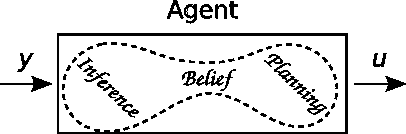
\includegraphics[height=0.7in]{agent}\qquad
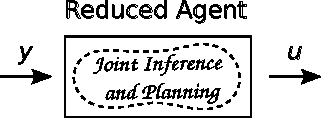
\includegraphics[height=0.7in]{reduced_agent}
\caption{\emph{Representation Reduction} Canonical belief spaces can become a serious informational bottleneck
between inference and planning modules.  
An agent's understanding of its environment need not be any richer than necessary
to support the task at hand.}
\end{figure}
\subsection{Previous Work}
The topic of reduction of logical functions has been extensively studied.
The formalism of finite state machines was developed in the 1950s and 60s,
and by 1971, Hopcroft \cite{hopcroft1971n} published an $(n\log n)$-time algorithm for 
reducing completely-specified FSMs. 
Incompletely-Specified FSMs were studied in turn, and various heuristics were 
developed to quickly approximate minimum\footnote{Here, we distinguish ``minimal'' from ``minimum'' reductions.  
A minimal reduction is one that cannot be further reduced by combining any of its states, whereas
a minimum reduction is a minimal reduction with the fewest possible states} 
 reductions. \cite{Pfleeger:1973:SRI:1311965.1312829,grasselli1965method,goren2007state}.
 Representation reduction in artificial intelligence has been dealt with in various guises:
 Dimensionality reduction, belief space compression etc.\ -- most heuristics can be considered as
 implicit hard-coded representation reductions.
\subsection{Contributions}
This chapter re-casts problem of representation reduction in terms of well-studied computational constructs,
and finds absolute minimum reductions in the case of discrete time, discrete input and output.
It evaluates three algorithms for approximating minimum reductions, and clarifies their strengths and weaknesses.
This work is the result of a collaboration of Andrea Censi, 
who introduced the formalism of representation reduction in the context of POMDP solvers
and proposed the bit-at-a-time algorithm
\section{Formalization}
\iffalse
\begin{definition}[Finite State Machine]
 A finite state machine is a tuple
 $$\ang{\Sigma, \Gamma, S, S_0, \delta, \omega},$$
 where $\Sigma$ and $\Gamma$ are finite input and ouput alphabets, $S$ is a finite set of states, $s_0\in S$ is an initial state,
 $\delta:S\times\Sigma\to S$ is a state-transition function, and $\omega:S\times\Sigma\to\Gamma$ is an output function.
\end{definition}
This generalizes to
\begin{definition}[Incompletely-Specified Finite State Machine (ISFSM)]
 An incompletely-specified finite state machine is a tuple
$$\ang{\Sigma, \Gamma, S, s_0 , \delta, \omega},$$
where $\Sigma$ and $\Gamma$ are finite input and ouput alphabets, $S$ is a finite set of states, $s_0\in S$ is an initial state,
 $\delta:S\times\Sigma\to S\cup\{\phi\}$ is a state-transition function, and $\omega:S\times\Sigma\to\Gamma\cup\{\epsilon\}$ is an output function.
The extra symbols $\phi\notin S$ and $\epsilon\notin\Gamma$ denote ``unspecified'' outputs, 
whose associated input and state are not expected to occur.
s\end{definition}
\begin{definition}[Policy]
 A decision policy is a tuple
 $\ang{\C,\U,T,\Y}$, where $\U$ is a set of actions, $\Y$ is a set of observations, $\C$ is a set of ``contexts'', (usually taken as the set of finite sequences in $\Y$), and
 and $T:(\C\times\Y)\to \U\cup\{\epsilon\}$ is a ``decision table'', assigning an action to each possible observation, for each context $c\in\C$.  
 Again $\epsilon$ is assigned to unexpected combinations of observation and context.
\end{definition}
\begin{definition}[Obedience]
Given the decision policy $P = \ang{\U, T : \operatorname{Sequences}(\Y)\to\U\cup\{\epsilon\}}$, we say
that an ISFSM $\ang{\Sigma, \Gamma, S, s_0, \delta, \omega}$ obeys the policy $P$ if for every finite
sequence $y_1, \ldots, y_n \in \Y$, there exists a sequence $s_0, \ldots, s_{n−1} \subs S$ such that
$s_i = \delta(s_{i−1} , y_i)$ for all $i = 1, \ldots, n$
and
$T(y_1, \ldots, y_n ) = \omega(s_{n−1} , y_n$
or
$T (y_1 , ... , y_n ) = \epsilon$.
\end{definition}


\begin{example}[Equivalent Decision Tables] \label{ex:complete}
Suppose $\Y=\{1,2\}$, $\U=\{A,B\}$, $\C=\bigcup_{i=1}^2\Y^i$ and 
$$\T(c) = \begin{cases}
A & c \in \{(1), (1,2)\}\\
B & c \in \{(2), (2,1)\}\\
\tT(c) & \text{otherwise.}
\end{cases},$$
is an optimal policy, for arbitrary $\tT:\C\to\U$. However, depending on the choice of $\tT$ (highlighted in the tables below),
the completed policy can have differently-sized minimal representations:

\begin{figure}[h]
\begin{floatrow}
\subfigure[Decision Table]{
\ffigbox[\FBwidth]{
\begin{tabular}{ll}
\rlap{$\T:\C\to\U$}\\
\hline
$(1)$&$\mapsto A$\\
$(2)$&$\mapsto B$\\
\rowcolor{Gray}
$(1,1)$&$\mapsto A$\\
$(1,2)$&$\mapsto A$\\
$(2,1)$&$\mapsto B$\\
\rowcolor{Gray}
$(2,2)$&$\mapsto B$
\end{tabular}
}{}}\quad
\subfigure[Decision Tree]{
\ffigbox[\FBwidth]{
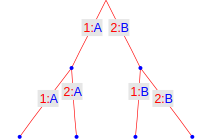
\includegraphics[scale=\sscale]{media/overcomplete_decision}
}{}}\quad\quad
\subfigure[Minimal Policy]{
\ffigbox[\FBwidth]{
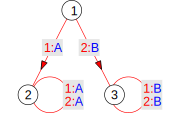
\includegraphics[scale=\sscale]{media/overcomplete-2}
}{}}
\end{floatrow}
\bigskip

\begin{floatrow}
\subfigure[Decision Table]{
\ffigbox[\FBwidth]{
\begin{tabular}{ll}
\rlap{$\T:\C\to\U$}\\
\hline
$(1)$&$\mapsto A$\\
$(2)$&$\mapsto B$\\
\rowcolor{Gray}
$(1,1)$&$\mapsto B$\\
$(1,2)$&$\mapsto A$\\
$(2,1)$&$\mapsto B$\\
\rowcolor{Gray}
$(2,2)$&$\mapsto A$
\end{tabular}
}{}}\quad
\subfigure[Decision Tree]{
\ffigbox[\FBwidth]{
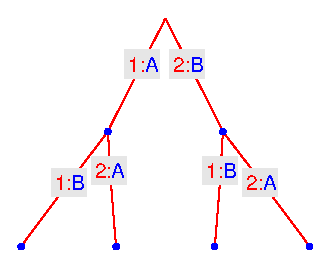
\includegraphics[scale=\sscale]{media/complete_decision}
}{}}\quad\quad
\subfigure[Minimal Policy]{
\hspace{.2cm}
\ffigbox[\FBwidth]{
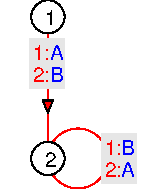
\includegraphics[scale=\sscale]{media/complete-2}
\setcounter{figure}{\value{example}}
\label{fig:best_completion}
}{}}
\end{floatrow}
\end{figure}
\end{example}
Instead, we propose an ``incompletely-determined'' formalization:
\fi
\begin{definition}[Policies]
Given a set $\Y$ of observations, recursively construct
\begin{equation}
\C_0 = \{\emptyset\}\qtx{and}\C_{i+1} = \{(c,y_{i+1})\,:\,c\in\C_i,\, y_{i+1}\in\Y_c\},
\end{equation}
where $\Y_c\subseteq\Y$ are the observations that may be seen in context $c$.  
Let $\C = \bigcup_{i=0}^{\infty}\C_i$.
A \textbf{policy} $P$ is then a tuple $\ang{\C, \U, \T, \Y}$, 
where $\U$ is some decision set and $\T:\C\andn\{\emptyset\}\to\U$.
\end{definition}
\begin{definition}[Completely-Determined Policies]
If $\Y=\bigcup_\C\Y_c$ and $\C=\Y^{\leq n}$ for some $n\in\NN$, then $P=\ang{\C,\U,\T,\Y}$ is \textbf{completely determined}.
A \textbf{completion} of $P$ is a policy $P\1=\ang{\C\1, \U\1, \T\1, \Y}$ such that
\begin{equation}
\Y\subseteq\Y\1,\quad \C\1=\bigcup_{i=0}^{\infty}(\Y\1)^i,\quad \U\subseteq\U\1, \qtx{and} \T\1|_{\C} = \T.
\end{equation}
Let $\Comp(P)$ be the set of completions of the policy $P$.
\end{definition}
\begin{definition}[FSM Representations]
An \textbf{FSM representation} (or just \textbf{representation})
is a tuple $\ang{\C,\R,\U,\S,\T,\Y}$ (abbreviated to $\ang{\R,\S}$ when $P=\ang{\C,\U,\T,\Y}$ is given), 
with ``states'' $\S\subseteq\NN$ and state assignments $\R:\C\to\S$, such that 
\begin{equation}
\R(c)=\R(c\1)\qtx{and}y\in\Y_c\cap\Y_{c\1}\implies\T(c,y)=\T(c\1,y).
\end{equation} 
Let $\Rep(P)$ be the set of representations of the policy $P$.  
\end{definition}
\begin{definition}[Minimal Representations]
The \textbf{size} of an FSM representation is the cardinality of its state set.  
A representation $\ang{\R,\S}$ of $P$ is \textbf{minimal} if 
$|\S|=\min\{|\S\1|\,:\,\ang{\R\1,\S\1}\in\Rep(P)\}$.
A representation $\ang{\R\1,\S\1}$ is a \textbf{reduction} of the representation $\ang{\R,\S}$ if there is a surjection $\phi:\S\to\S\1$
such that $\R\1 = \phi(\R)$.
\end{definition}
\begin{example}
\label{ex:canon}
If $\C = \{c_1, c_2, \ldots\}$, then 
%for any policy $P=\ang{\C,\U,\T,\Y}$,
we have a canonical representation $\ang{\R,\S}$, where
\begin{equation}
\S=\{1,\ldots,|\C|\}\qtx{and}\R:c_k\mapsto k.
\end{equation} 
\end{example}
It can be shown that the size of a minimal representation of a policy $P$ is equal to the minimum
size of the minimal representations of its completions, i.e.
\begin{align}
\min\{|\S\1|\,:\,\ang{\R\1,\S\1}\in\Rep(P)\} = \min\{|\S\1|\,:\,\ang{\R\1,\S\1}\in\Rep(P\1),\,P\1\in\Comp(P)\}
\end{align}
Incompletely-determined policies allow more freedom in representation reduction, as shown in the next example.

\begin{example}[Incompletely-Determined Policies]
Let $\C=\{\emptyset, (1), (2), (1,2), (2,1)\}$, $\U=\{A,B\}$, and
\begin{equation*}
\T(c,y) = \begin{cases}
A & c\in\{(1), (1,2)\}\\
B & c\in\{(2), (2,1)\}
\end{cases}.
\end{equation*}
Observe that the minimal policy is the same as that of the completely-determined policy in Example \ref{fig:best_completion}.
\setcounter{subfigure}{0}
\begin{figure}[h]
\begin{floatrow}
\subfigure[Decision Table]{
\ffigbox[\FBwidth]{
\begin{tabular}{ll}
\multicolumn{2}{c}{$\T:\C\andn\{\emptyset\}\to\U$}\\
\hline
$(1)$&$\mapsto A$\\
$(2)$&$\mapsto B$\\
$(1,2)$&$\mapsto A$\\
$(2,1)$&$\mapsto B$\\
\end{tabular}
}{}}
\subfigure[Decision Tree]{
\ffigbox[\FBwidth]{
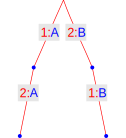
\includegraphics[scale=\sscale]{media/simple_decision}
}{}}\qquad
\subfigure[Representation]{
\ffigbox[\FBwidth]{
\begin{tabular}{ll}
\rlap{$\R:\C\to\S$}\\
\hline
$\emptyset$&$\mapsto 1$\\
$(1)$&$\mapsto 2$\\
$(2)$&$\mapsto 2$\\
$(1,2)$&$\mapsto 2$\\
$(2,1)$&$\mapsto 2$\\
\end{tabular}
}{}}
\subfigure[Minimal Policy]{
\ffigbox[\FBwidth]{
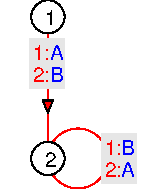
\includegraphics[scale=\sscale]{media/complete-2}
}{}}
\end{floatrow}
\setcounter{figure}{\value{example}}
\label{fig:incomplete}
\end{figure}
\end{example}
\subsection{FSM Reduction}
Given a decision policy (or an ISFSM) how do we find an obedient (or
equivalent) ISFSM with the smallest possible state set?

for completely-specified FSM, this can be done in $n\log n$ time
by Hopcroft's algorithm (Alg.\ \ref{algo: Hopcroft}).


To find a minimum representation of a given policy,
we first compute a graph of reducibility relations, 
then compute a minimal clique-covering.

Cliques on the equivalence graph identify sets of states that can be
collapsed into a single state. The minimal clique-covering, that is the
smallest collection of disjoint cliques that covers the equivalence
graph, correponds to a minimal reduction of the FSM.

\section{Representation Reduction Strategies}


\setcounter{subfigure}{0}
\begin{figure}[ht]
\centering
\subfigure[Canonical Representation]{
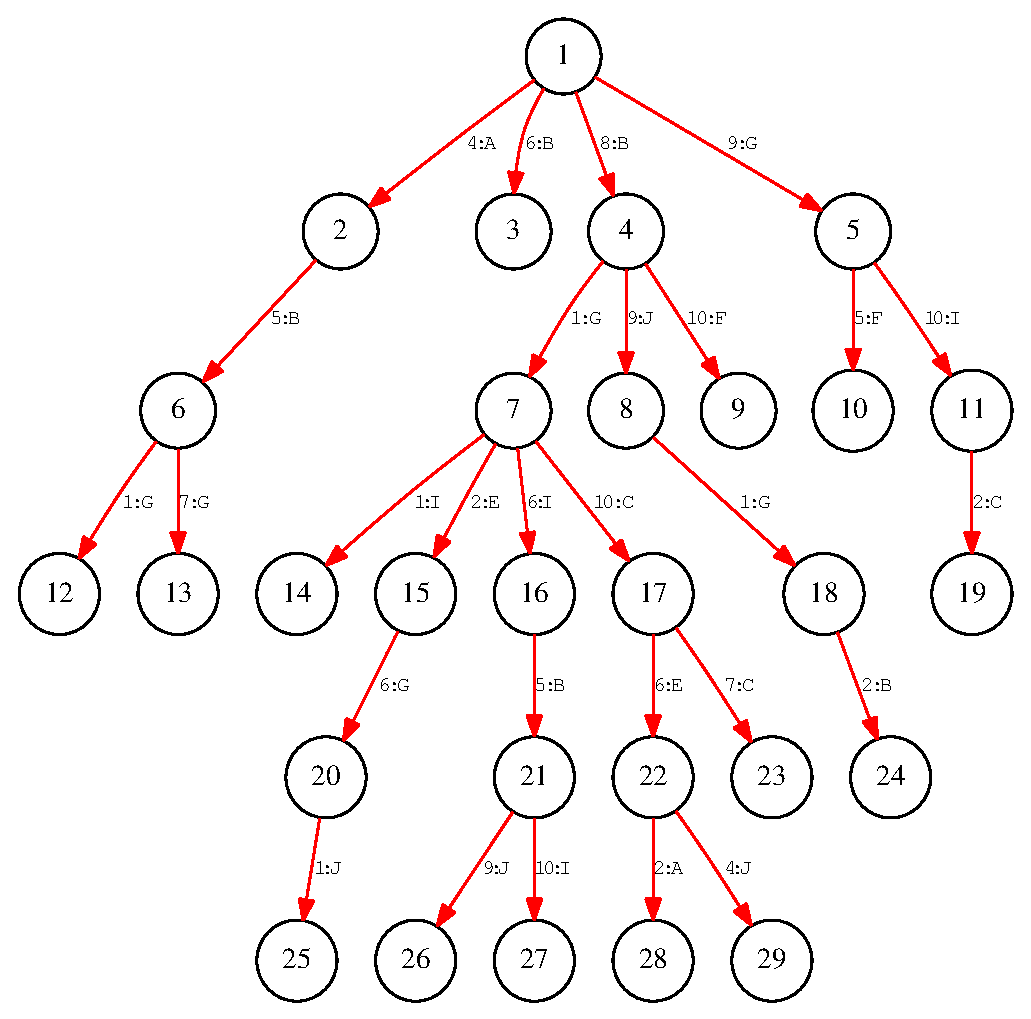
\includegraphics[height=\bfigh]{media/random_alg-1}}\qquad
\subfigure[Compatibility Matrix]{\label{fig:cgam}
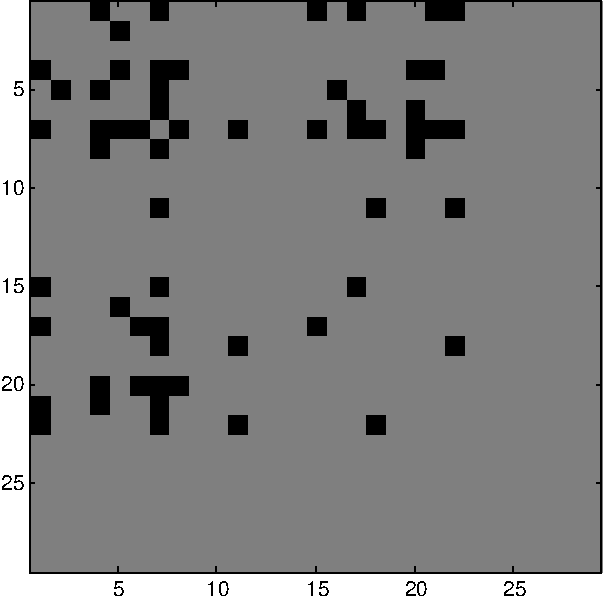
\includegraphics[height=\bfigh]{media/random_adj}}
\end{figure}

\begin{figure}[ht]
\subfigure[Greedy Clique Covering of \ref{fig:cgam}]{
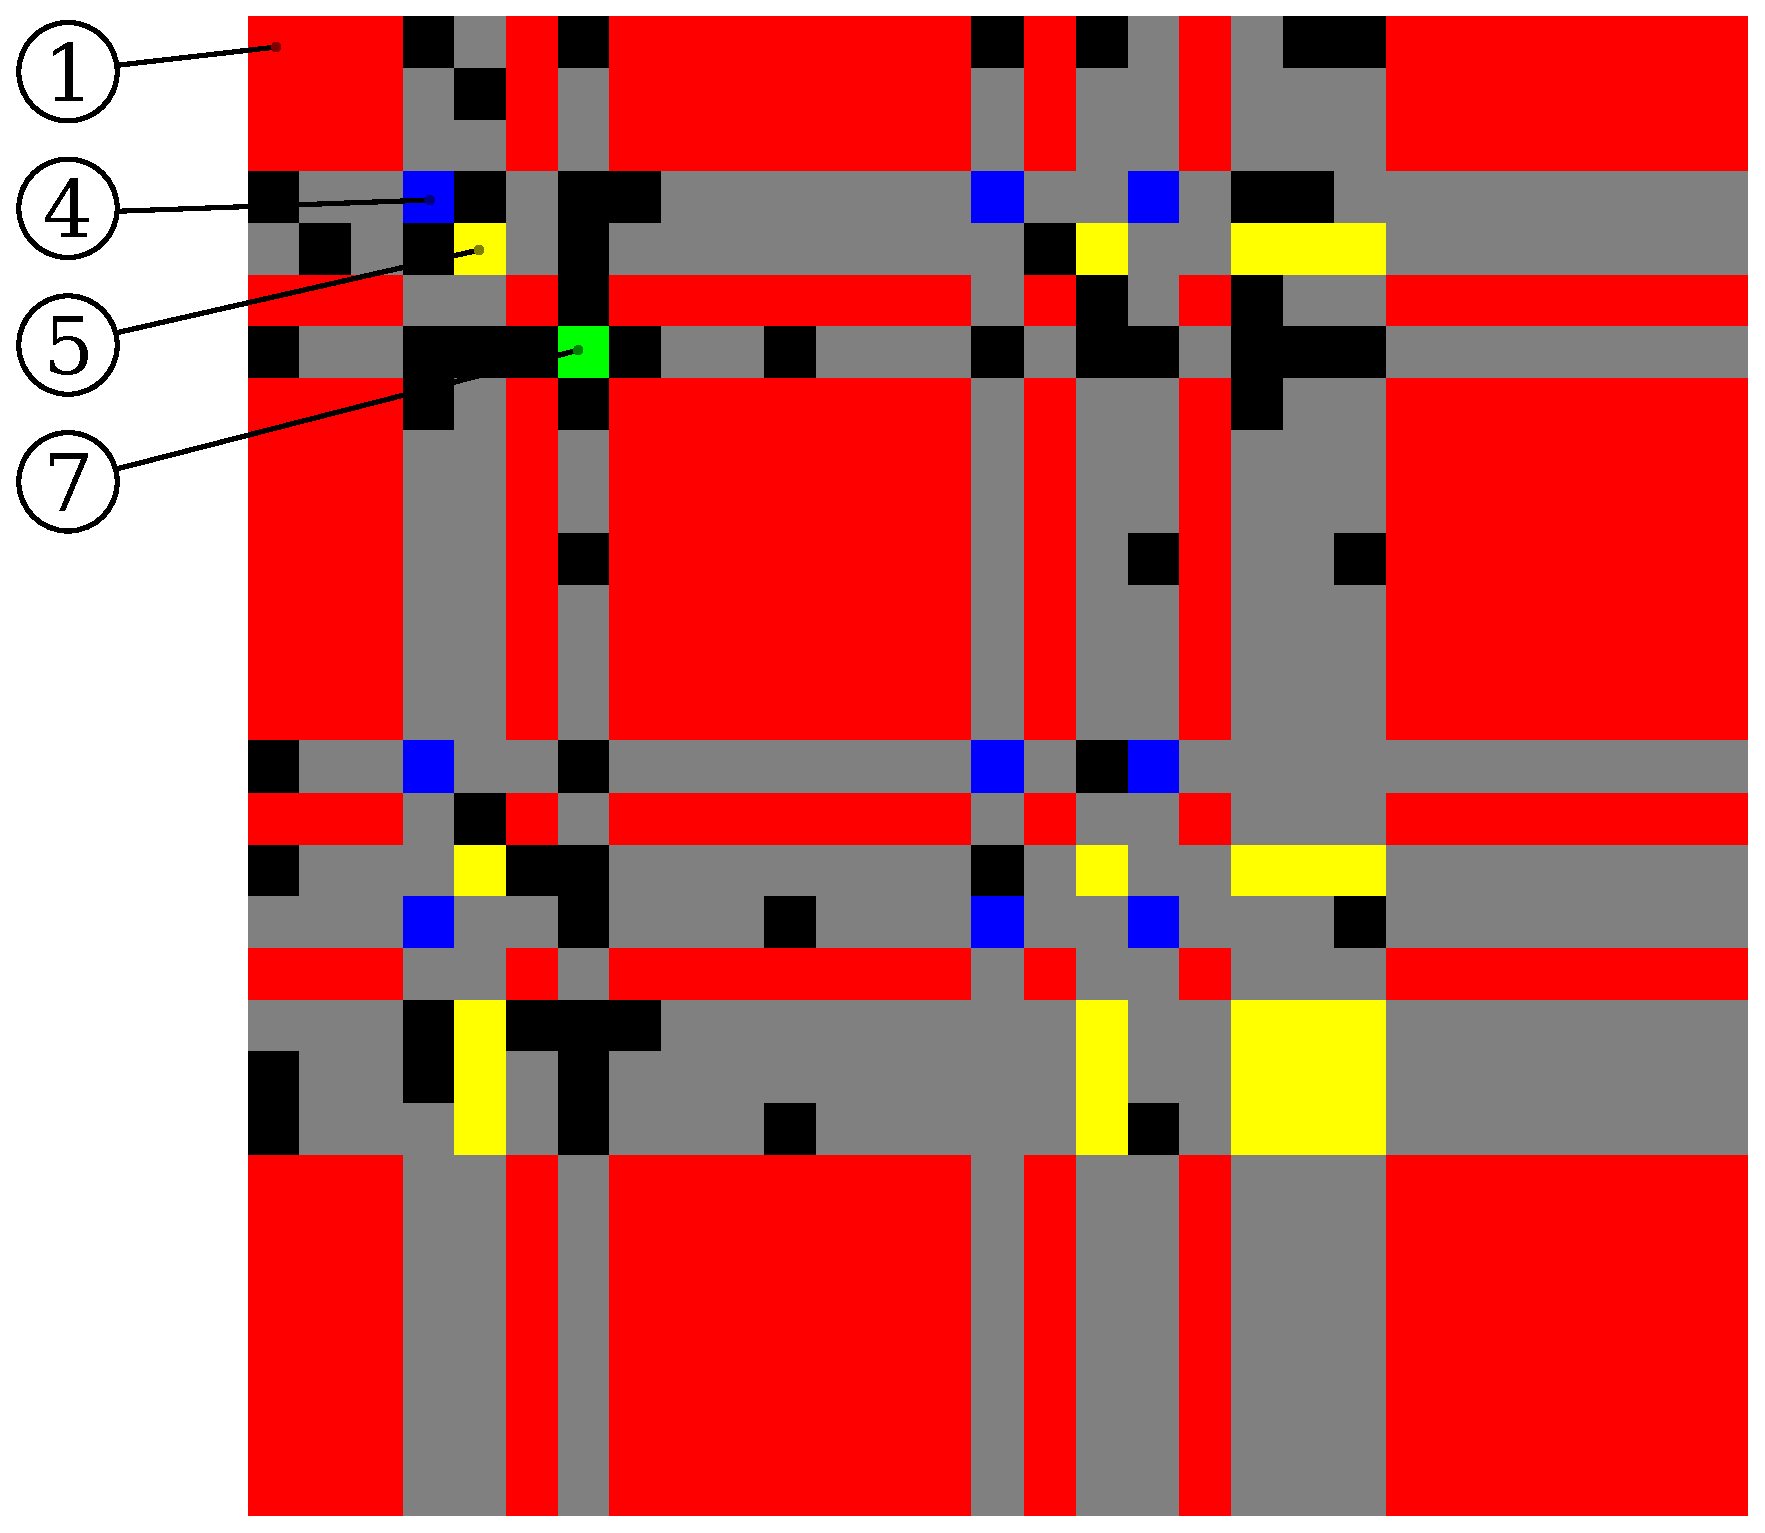
\includegraphics[height=\bfigh]{media/random_cliques}}
\qquad
\subfigure[Reduced Representation]{
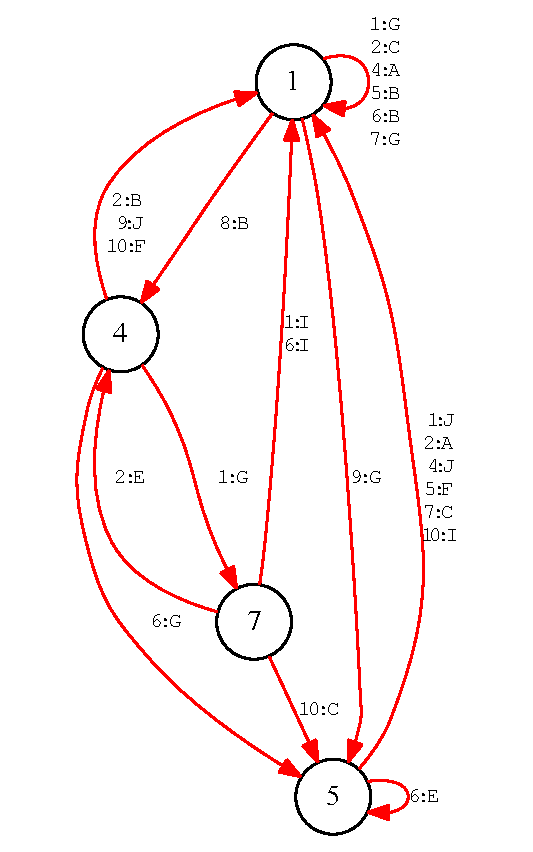
\includegraphics[height=\bfigh]{media/random_alg-2}}
\caption{\emph{Greedy Reduction Algorithm} A ``running clique'' is kept, to which new states are added until all remaining states are
incompatible with at least one state in the clique.  Then, a new clique is begun.  
Here, the cliques are 
$\{1, 2, 3, 6, 8, 9, 10, 11, 12, 13, 14, 16, 19, 22, 26, 27, 28, 29, 30, 31, 32\}$ (red),
$\{4, 15, 18\}$ (blue), $\{5, 17, 21, 22, 23\}$ (yellow), and $\{7\}$ (green). (d) shows the resulting policy graph once 
}
\end{figure}
For practical computation of reducibility, we'll start with the weaker condition of compatibility.

\subsection{Reducibility Relations}

\begin{definition}[Reducibility]
For a given policy $P=\ang{\C,\U,\T,\Y}$, two contexts $c_1, c_2\in\C$ are \textbf{reducible} (write $c_1\sim c_2$) if there exists a representation 
$\ang{\R,\S}$ of $P$ such that $\R(c_1)=\R(c_2)$.  Likewise, for a given representation $R=\ang{\R,\S}$, two states 
$s_1,s_2\in\S$ are \textbf{reducible} if there exists a reduction $(\phi, \ang{\R\1,\S\1})$ of $R$ such that
$\phi(s_1)=\phi(s_2)$.
\end{definition}
Observe that for any representation $\ang{\C,\R,\U,\S,\T,\Y}$,
the contexts $c_1, c_2\in\C$ are reducible if and only if the states $\R(c_1)$ and $\R(c_2)$ are reducible.
Observe also that for incompletely-determined policies, reducibility is a symmetric but not-necessarily-transitive relation
\begin{example}[Non-Transitive Reducibility]
Suppose $\Y=\{1,2,3\}$, $\C=\{\emptyset, (1), (2), (1,3), (2,3)\}$, \mbox{$\U=\{A,B\}$}, and 
\begin{equation}
\T(c) = \begin{cases}
A&c\in\{(1), (1,3)\}\\
B&c\in\{(2), (2,3)\}
\end{cases}.
\end{equation} 
Observe that, under this policy, $\emptyset\sim(1)$ and $\emptyset\sim(2)$, but $(1)\not\sim(2)$, 
since $\T(1,3)\neq\T(2,3)$.
\end{example}
However, it can be shown that, under a completely-determined policy, reducibility induces an equivalence relation.  
In either case, we compute reducibility using the following criterion:
\begin{lemma}
Two contexts $c_1,c_2\in\C$ are reducible iff 
\begin{equation}
\T(c_1,s)=\T(c_2,s)\qtx{for all}s\in\Y^*\qtx{such that}(c_1,s),(c_2,s)\in\C
\end{equation} 
\end{lemma}

This informs the following algorithm
\begin{algorithm}                      % enter the algorithm environment
\label{algo: Hopcroft}
\caption{(Hopcroft) Compute Reducibility Relations}          % give the algorithm a caption
\label{alg1}                           % and a label for \ref{} commands later in the document
\begin{algorithmic}                    % enter the algorithmic environment
  \REQUIRE A representation $\ang{\C,\R,\U,\S,\T,\Y}$
  \ENSURE A reducibility matrix $A:\S\times\S\to\{\TRUE,\FALSE\}$.
  \bigskip
  
  \STATE $A(s_1, s_2)\Leftarrow \TRUE$\quad for all $s_1,s_2\in\S$.
  \REPEAT
    \STATE $isChanged \Leftarrow \FALSE$
    \FOR{$s_1<s_2\in \S$}
	  
	  \IF{$A(s_1,s_2)=\TRUE$}
		\FOR{$c_1\in\R\inv(s_1),\,c_2\in\R\inv(s_2)$}
		  \FOR{$y\in\Y_{c_1}\cap\Y_{c_2}$}
			\IF{$\T(c_1,y)\neq\T(c_2,y)\;\;\text{or}\;\;^{\sim}A(\R(c_1,y),\R(c_2,y))$}
			  \STATE $A(s_1,s_2)\Leftarrow\FALSE$.
			  \STATE $isChanged\Leftarrow\TRUE$.
			\ENDIF
		  \ENDFOR
		\ENDFOR
	  \ENDIF
    \ENDFOR
  \UNTIL{$^{\sim}isChanged$} 
\end{algorithmic}
\end{algorithm}

\subsection{Bit-at-a-Time}
The Bit-at-a-Time reduction, proposed by Andrea Censi, generates a set of states one at a time,
separating ambiguous contexts recursively.  An ambiguous context is an (input, state) pair for
which more than one output is defined.  Ambiguities which arise in shorter sequences are separated first.
\begin{figure}
\centering
\subfigure[Decision Tree]{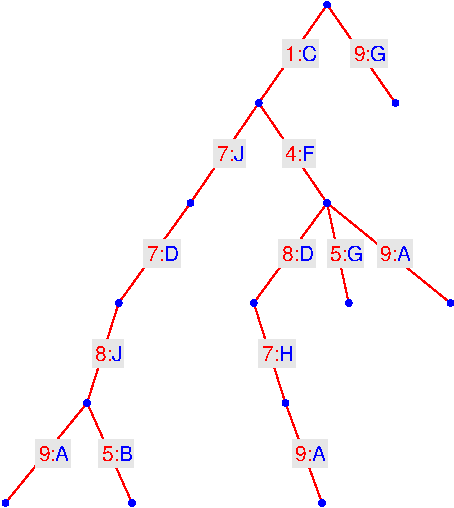
\includegraphics[height=2in]{cdiag1}}
\subfigure[Partitioned Tree]{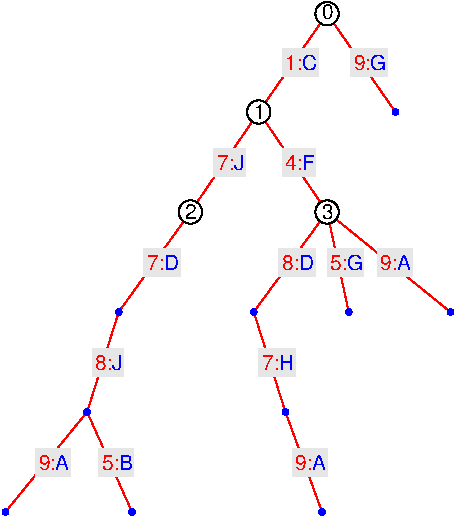
\includegraphics[height=2in]{cdiag2}}
\subfigure[Reduced FSM]{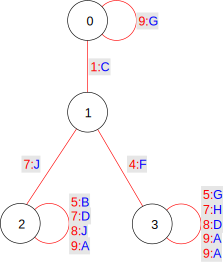
\includegraphics[width=1in]{cdiag3}}
\caption{\emph{Censi's Bit-at-a-time Algorithm}}
\end{figure}
 
\subsection{Greedy Covering}

Although reducibility is not an equivalence relation, 
any reduction $\phi:\S\to\S\1$ induces an equivalence relation,
partitioning $\S$ into cliques of mutually-reducible states, i.e.
\begin{equation}
\S = \bigsqcup_{s\1\in\S\1}\phi\inv(s\1),\qtx{where}\phi(s_1)=\phi(s_2)\implies A(s_1,s_2)
\end{equation}
Thus, a minimum 
reduction
induces a minimum clique partition of the
reducible states of a representation.
\subsection{Assembling Cliques}
\begin{notation}[Arrow notation]
For a policy $P=\ang{\C,\U,\T,\Y}$, 
write $c\to c\1$ if $c=(c_1,\ldots,c_i)\in\C_i\subseteq\C$ and 
$c\1=(c_1,\ldots,c_i,y)\in\C_{i+1}\subseteq\C$, for some $i$.  For a representation $\ang{\R,\S}$ of $P$,
write $s_1\to s_2$ if there are $c_1\in f\inv(s_1)$ and $c_2\in f\inv(s_2)$ such that $c_1\to c_2$.
\end{notation}
We propose the following, greedy, approximate algorithm
\begin{algorithm}                      % enter the algorithm environment
\caption{Greedy Clique Covering}          % give the algorithm a caption
\label{alg2}                           % and a label for \ref{} commands later in the document
\begin{algorithmic}                    % enter the algorithmic environment]
  \REQUIRE A representation $\ang{\C,\R,\U,\S,\T,\Y}$ with $s_1<s_2$ only if $s_2\not\to s_1$.
  \REQUIRE A reducibility matrix $A:\S\times\S\to\{\TRUE,\FALSE\}$ as computed by Algorithm \ref{alg1}.
  \ENSURE A partition function $\phi:\S\to\S\1$ with $\phi(s_1)=\phi(s_2)$ only if $A(s_1,s_2)$.
  \bigskip
  
  \STATE $\S\1\Leftarrow\S$
  \STATE $\phi\Leftarrow id_{\S}$
  \STATE $unused\Leftarrow\S$
  \WHILE{$|unused|>0$}
	\STATE $s_1\Leftarrow\min(unused)$
	\STATE $unused\Leftarrow unused\andn\{s_1\}$
	\FOR{$s_2\in unused$}
	  \IF{$A(s_1,s_2)$}
		\STATE $\phi(s_2)\Leftarrow s_1$
		\STATE $unused\Leftarrow unused\andn\{s_2\}$
	  \ENDIF
	\ENDFOR
  \ENDWHILE
\end{algorithmic}
\end{algorithm}
In order find the absolute minimum representation of a
given policy, it suffices to run the greedy algorithm on all
possible orderings of its states: 
Given a minimum clique covering 
$S=\{s_{c_{11}}, s_{c_{12}}, \ldots, s_{c_{1 N_1}}\}$
$\cup$
$\{s_{c_{21}}, s_{c_{22}}, \ldots, s_{c_{2 N_2}}\}$
$\cup$ $\cdots$ $\cup$
$\{s_{c_{K1}}, s_{c_{K2}}, \ldots, s_{c_{K N_K}}\}$,
feed states to the greedy algorithm in the order in which they are written.
%i.e. add from the list $s_{c_{11}}, s_{c_{12}}, \ldots, s_{c_{1N_1}}, s_{c_{21}},\ldots$ until
Failure to add states to a running clique will occur only once per clique in the minimal covering (exactly $K$ times)
\footnote{If more than $K$ times, then some running clique },
so the greedy algorithm will produce a minimum covering.  Of course, 
exhaustively checking every ordering will end up taking exponential time.
In fact, it has been shown that the minimum clique cover problem is NP-hard \cite{karp72}.
\subsection{Maximal Anticlique}
Alberto and Sim\~ao \cite{4813796} propose a heuristic to 
increase the likelihood that a greedy algorithm produces a minimum clique covering --
First, a maximum anticlique is found in the compatibility graph (This is also an NP-hard problem \cite{karp72},
but the size of the maximum anticlique generally grows more slowly than the graph itself).
Now, each state in the maximum anticlique must belong to a different clique in the minimum
clique covering.  Also, every remaining state must be compatible with at least one of the states in the 
anticlique (or else violate the maximality of the anticlique).  The greedy algorithm then proceeds,
taking first the states in the maximum anticlique, then the remaining states
It can easily be shown that an ordering of this type will produce a 
minimum reduction.  The number of such orderings still grows exponentially with 
the number of states, but in practice it grows significantly more slowly.
\begin{figure}
\setcounter{subfigure}{0}
\centering
\subfigure[Bad Ordering]{
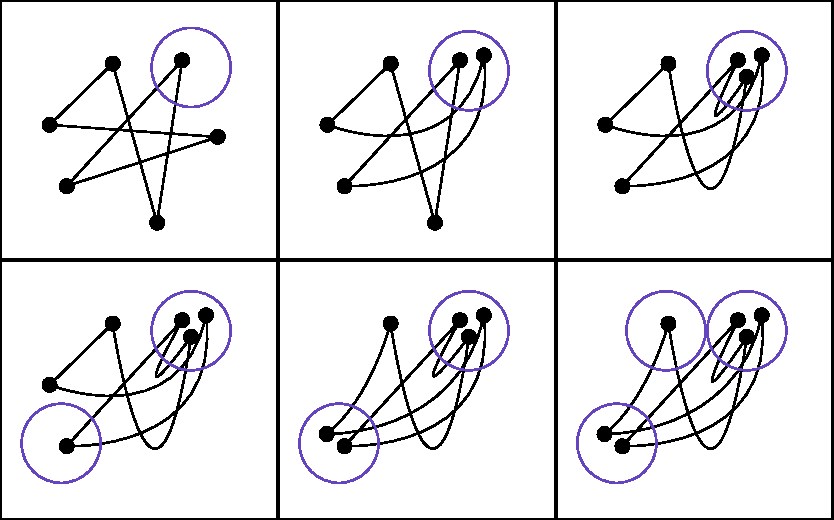
\includegraphics[width=4in]{bad_greedy.pdf}}
\subfigure[Good Ordering]{
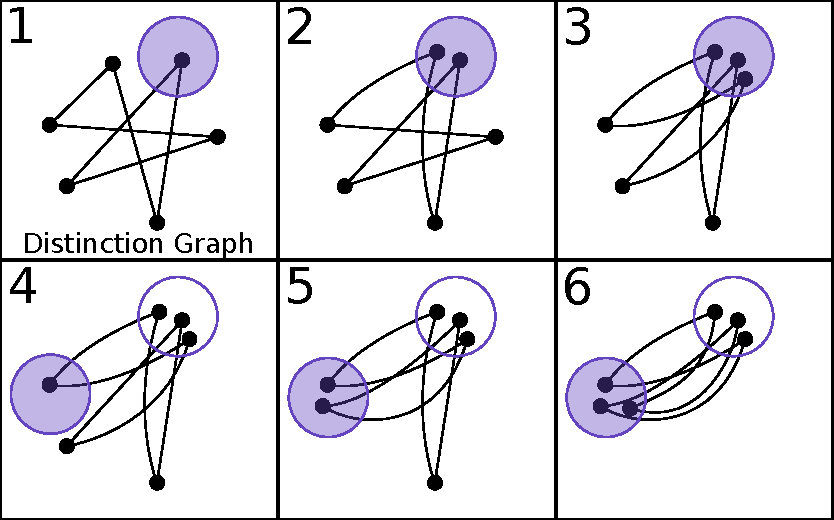
\includegraphics[width=4in]{good_greedy.pdf}}
\caption{\emph{Greedy Algorithm on Pathological Trees}
\label{goodbad_order}
Here we illustrate the dependence of greedy algorithms
on the order of their inputs.
In the first set of figures (a), we proceed randomly,
greedily adding random states to a running clique until none can be added
(no two states sharing an edge in the distinction graph can be part of the same clique).
This results in one more clique than is necessary - 
proceeding counterclockwise, we cover the set with only two cliques.
Alberto and Sim\~ao's
maximum anticlique algorithm
fares no better, as the maximal anticlique has size 2.
}
\end{figure}

\subsection{Comparisons}
Two types of random FSMs were generated to test the correctness and numerical efficiency of the 
algorithms described above.
\subsubsection{Poisson Random Tree}
A Poisson random tree is an decision policy generated by recursively adding
      $X\sim\operatorname{Poisson(\lambda)}$ children to each new node of 
      an existing policy.
      We conditioned this result on the outcome that the  process not terminate before the tree 
      reaches depth $H$ (contains a sequence of length $H$ or greater).
      These decision policies are well-studied in decision theory, as they model birth/death processes where
      individuals continuously produce
      offspring at a rate of $\lambda$ per lifetime.
\begin{figure}
\centering
\subfigure[Poisson Tree Growth Trend]{
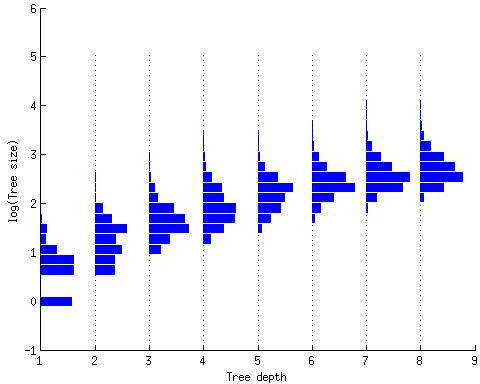
\includegraphics[height=1.8in]{poiss_size.jpg}\qquad
}
\subfigure[Tree, Depth 10]{
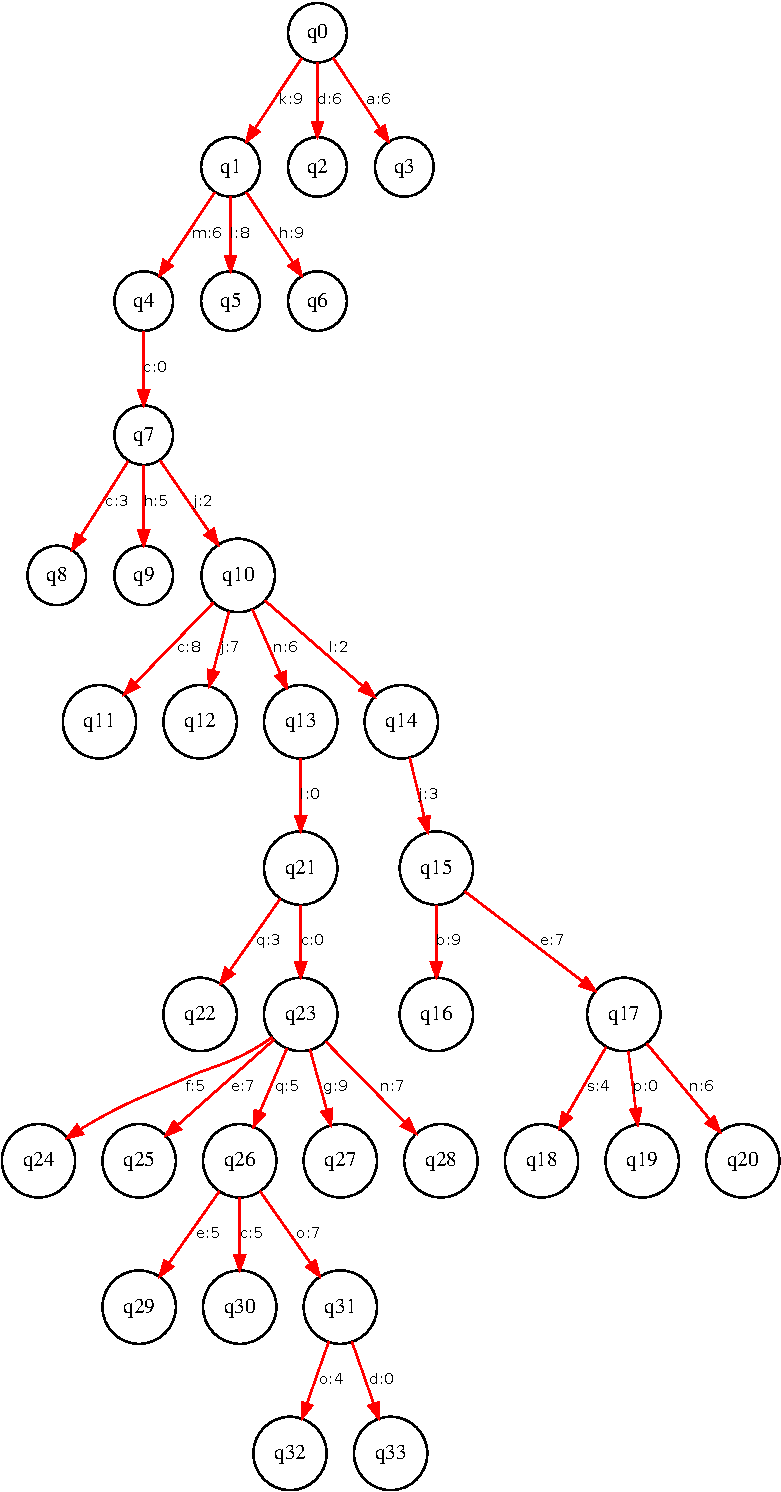
\includegraphics[height=1.8in]{big_tree_left.pdf}}
\caption{\emph{Poisson Random Tree}}
\end{figure}
\subsubsection{Pathological Tree}
The ``pathological'' tree is a policy of depth 2 with $6n+1$ contexts.
was designed to frustrate the algorithm of Alberto and Sim\~ao.
Each of its states at depth 1 is incompatible with exactly two others.  
The resulting distinction graph consists of disjoint rings. 
The order in which states are added to cliques is critical.  
Half of all orderings result in a three-state FSM, whereas the minimum number of states is two.
\begin{figure}
\centering
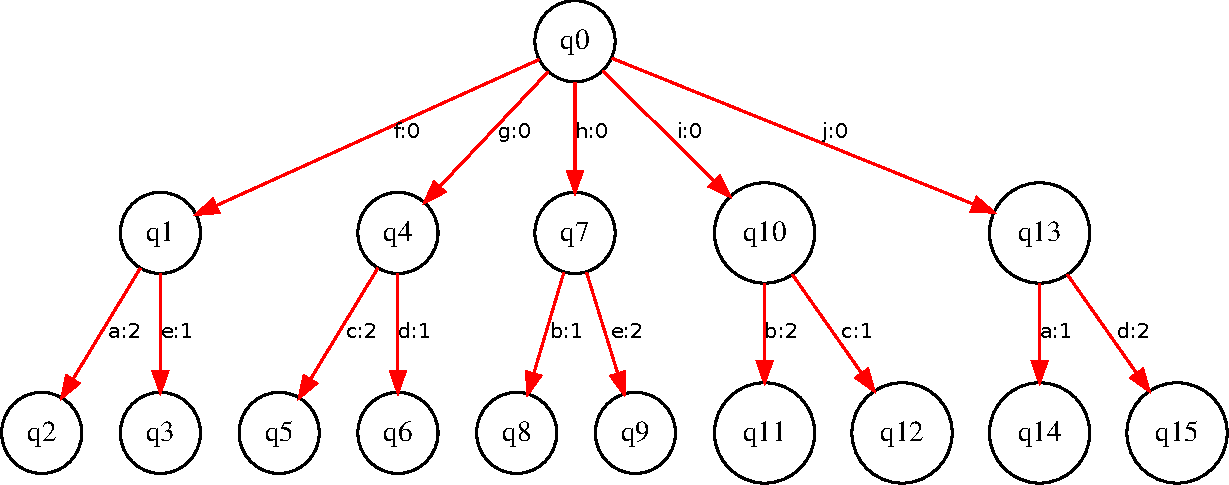
\includegraphics[width=4in]{big_patho_tree.pdf} 
\caption{\emph{Pathological Tree} }
\end{figure}
\begin{figure}
\centering
\subfigure[\scriptsize{Original}]{
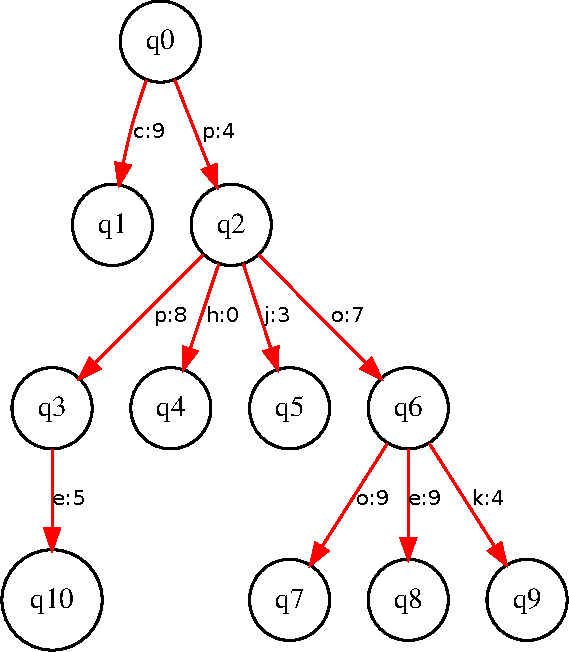
\includegraphics[scale=0.25]{orig.pdf}
}
\subfigure[\scriptsize{Bit-at-a-Time}]{
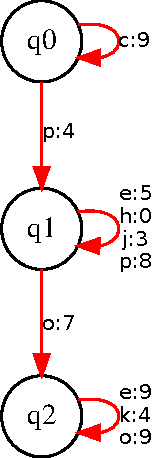
\includegraphics[scale=0.3, angle=35]{censi.pdf}
}
\subfigure[\scriptsize{Greedy}]{
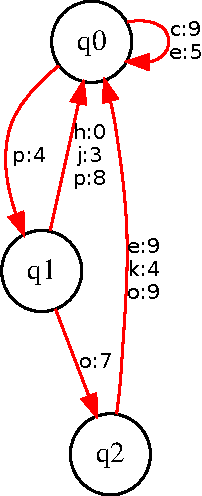
\includegraphics[scale=0.3, angle=35]{josh.pdf}
}
\subfigure[\scriptsize{Alberto-Sim\~ao}]{
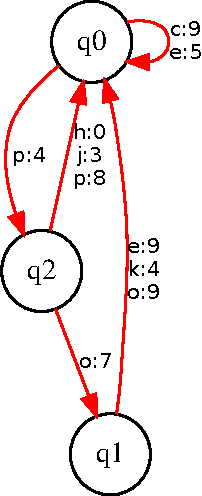
\includegraphics[scale=0.3, angle=35]{alberto.pdf}
}
\subfigure[\scriptsize{Exact}]{
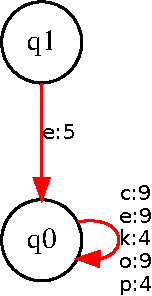
\includegraphics[scale=0.3, angle=35]{exact.pdf}
}
\caption{\emph{Typical Reductions}
Here we contrast the results of the various reduction algorithms introduced above.
The Bit-at-a-Time method (b) produces a minimal sub-tree of
the canonical policy.
The last three methods are equivalent up to a reordering of states,
so reductions (c) and (d) are practically identical. 
}
\end{figure}
\section{Discussion}

\begin{figure}
\centering
\subfigure[Poisson Trees Reduced vs.\ Orig.\ Size]{
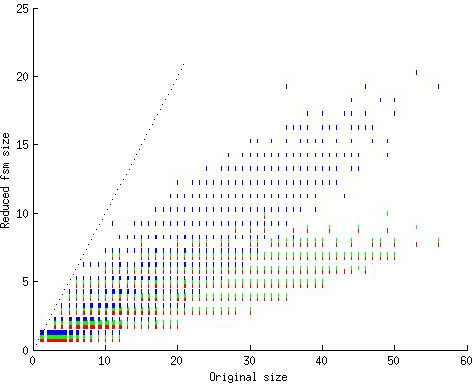
\includegraphics[height=1.7in]{poiss_orig.jpg}}\qquad
\subfigure[Patho.\ Trees Reduced vs.\ Orig.\ Size]{
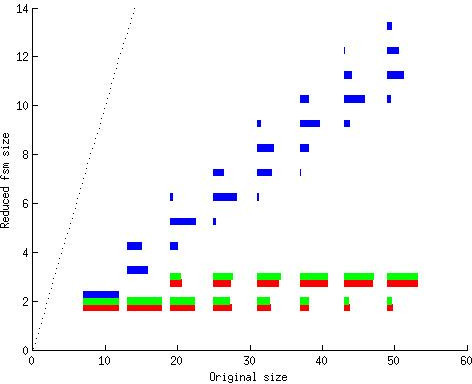
\includegraphics[height=1.7in]{patho_orig.jpg}}\\
\subfigure[Poisson Trees Reduced vs.\ Min.\ Size]{
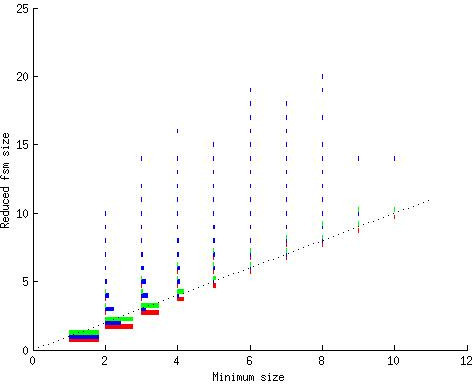
\includegraphics[height=1.7in]{poiss_exact.jpg}}\qquad
\subfigure[Patho.\ Trees Reduced vs.\ Min.\ Size]{
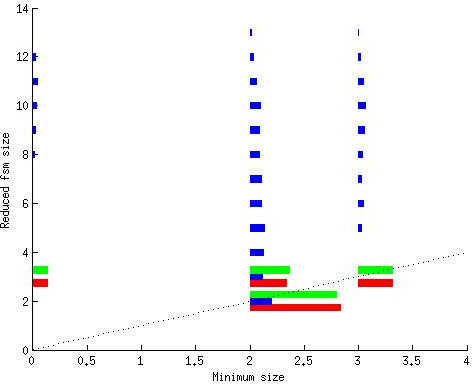
\includegraphics[height=1.7in]{patho_exact.jpg}}\\
\subfigure[Algo.\ Runtimes on Poison Trees]{
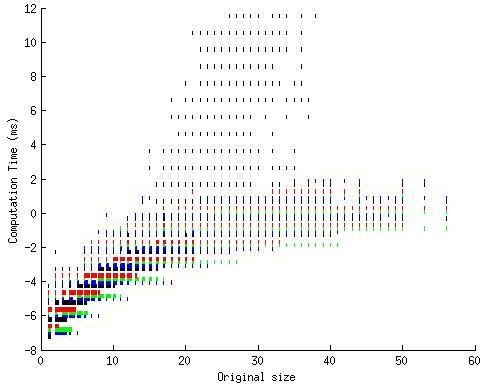
\includegraphics[height=1.7in]{poiss_time.jpg}}\qquad
\subfigure[Algo.\ Runtimes on Patho.\ Trees]{
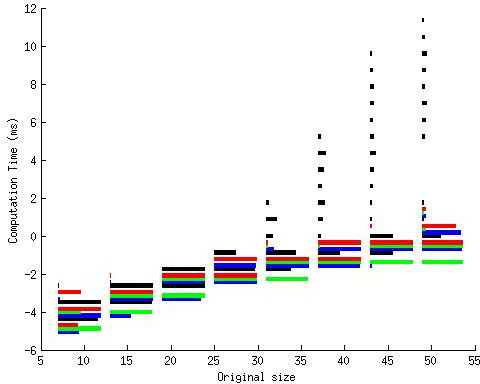
\includegraphics[height=1.7in]{patho_time.jpg}}
\caption{\emph{} {Red} bars pertain to Alberto and Sim\~ao's method, 
{blue} bars pertain to the bit-at-a time method, 
{green} bars pertain to the greedy clique completion method, 
and
{black} bars pertain to an exhaustive search for a minimal reduction.
}
\end{figure}



\bibliographystyle{plain}
\bibliography{Exploration/exploration.bib,Exploration/text.bib,Observability/self.bib,Observability/filter.bib,Observability/total2.bib,SolidObjects/cvpr2015_solobj/bib/solidObjDet.bib,SolidObjects/cvpr2015_solobj/bib/solidObjDet2.bib,SolidObjects/cvpr2015_solobj/bib/taylorARS12.bib,SolidObjects/cvpr2015_solobj/bib/ayvaciS13.bib,SolidObjects/cvpr2015_solobj/bib/ayvaciS11mdl.bib,SolidObjects/cvpr2015_solobj/bib/trevor.bib,MinRep/minrep.bib}
\end {document}

